\documentclass{article}
% Packages
\usepackage{amssymb,amsmath,amsthm,bbm}
\usepackage{verbatim,float,url,dsfont}
\usepackage{graphicx,subcaption,psfrag}
\usepackage{algorithm,algorithmic}
\usepackage{mathtools,enumitem}
\usepackage{multirow}
\usepackage{ragged2e}
\usepackage{xr-hyper}
\usepackage{array}

\usepackage[colorlinks=true,citecolor=blue,urlcolor=blue,linkcolor=blue]{hyperref}
\usepackage[margin=1in]{geometry}
\usepackage[round]{natbib}

\usepackage[utf8]{inputenc} % allow utf-8 input
\usepackage[T1]{fontenc}    % use 8-bit T1 fonts
\usepackage{booktabs}       % professional-quality tables
\usepackage{nicefrac}         % compact symbols for 1/2, etc.
\usepackage{microtype}      % microtypography

\ifdefined\TimesFont 
\usepackage{times} % use times font
\fi

\ifdefined\ParSkip 
\usepackage{parskip} % use par skip
\fi

% Theorems and such
\newtheorem{theorem}{Theorem}
\newtheorem{lemma}{Lemma}
\newtheorem{corollary}{Corollary}
\newtheorem{proposition}{Proposition}
\theoremstyle{definition}
\newtheorem{remark}{Remark}
\newtheorem{definition}{Definition}

% Assumption
\newtheorem*{assumption*}{\assumptionnumber}
\providecommand{\assumptionnumber}{}
\makeatletter
\newenvironment{assumption}[2]{
  \renewcommand{\assumptionnumber}{Assumption #1#2}
  \begin{assumption*}
  \protected@edef\@currentlabel{#1#2}}
{\end{assumption*}}
\makeatother

% Widebar
\makeatletter
\newcommand*\rel@kern[1]{\kern#1\dimexpr\macc@kerna}
\newcommand*\widebar[1]{%
  \begingroup
  \def\mathaccent##1##2{%
    \rel@kern{0.8}%
    \overline{\rel@kern{-0.8}\macc@nucleus\rel@kern{0.2}}%
    \rel@kern{-0.2}%
  }%
  \macc@depth\@ne
  \let\math@bgroup\@empty \let\math@egroup\macc@set@skewchar
  \mathsurround\z@ \frozen@everymath{\mathgroup\macc@group\relax}%
  \macc@set@skewchar\relax
  \let\mathaccentV\macc@nested@a
  \macc@nested@a\relax111{#1}%
  \endgroup
}
\makeatother

% Operators and shortcuts
\DeclareMathOperator*{\argmin}{argmin}
\DeclareMathOperator*{\argmax}{argmax}
\DeclareMathOperator*{\minimize}{minimize}
\DeclareMathOperator*{\maximize}{maximize}
\DeclareMathOperator*{\find}{find}
\DeclareMathOperator{\st}{subject\,\,to}

\DeclareMathOperator{\Cor}{Cor}
\DeclareMathOperator{\Cov}{Cov}
\DeclareMathOperator{\Var}{Var}
\DeclareMathOperator{\dm}{dim}
\DeclareMathOperator{\col}{col}
\DeclareMathOperator{\row}{row}
\DeclareMathOperator{\nul}{null}
\DeclareMathOperator{\rank}{rank}
\DeclareMathOperator{\nuli}{nullity}
\DeclareMathOperator{\spa}{span}
\DeclareMathOperator{\sign}{sign}
\DeclareMathOperator{\supp}{supp}
\DeclareMathOperator{\diag}{diag}
\DeclareMathOperator{\aff}{aff}
\DeclareMathOperator{\conv}{conv}
\DeclareMathOperator{\dom}{dom}
\DeclareMathOperator{\tr}{tr}
\DeclareMathOperator{\df}{df}

\def\E{\mathbb{E}}
\def\P{\mathbb{P}}
\def\R{\mathbb{R}}
\def\C{\mathbb{C}}
\def\N{\mathbb{N}}
\def\Z{\mathbb{Z}}
\def\T{\mathsf{T}}

\def\half{\frac{1}{2}}
\def\df{\mathrm{df}}
\def\hy{\hat{y}}
\def\hf{\hat{f}}
\def\hmu{\hat{\mu}}
\def\halpha{\hat{\alpha}}
\def\hbeta{\hat{\beta}}
\def\htheta{\hat{\theta}}
\def\indep{\perp\!\!\!\perp}
\def\th{^{\textnormal{th}}}

\def\cA{\mathcal{A}}
\def\cB{\mathcal{B}}
\def\cD{\mathcal{D}}
\def\cE{\mathcal{E}}
\def\cF{\mathcal{F}}
\def\cG{\mathcal{G}}
\def\cK{\mathcal{K}}
\def\cH{\mathcal{H}}
\def\cI{\mathcal{I}}
\def\cL{\mathcal{L}}
\def\cM{\mathcal{M}}
\def\cN{\mathcal{N}}
\def\cP{\mathcal{P}}
\def\cS{\mathcal{S}}
\def\cT{\mathcal{T}}
\def\cW{\mathcal{W}}
\def\cX{\mathcal{X}}
\def\cY{\mathcal{Y}}
\def\cZ{\mathcal{Z}}

\usepackage{graphicx} % Required for inserting images
\usepackage{dsfont}
\usepackage{amsfonts}
\usepackage{amsmath}
% \usepackage[authoryear,sort&compress]{natbib}
% \usepackage[numbers, sort]{natbib}
% \usepackage{hyperref}
\usepackage{caption}
\usepackage{subcaption}

\title{Challenges in Real-Time Estimation of Changing Epidemic Severity Rates}
\author{Jeremy Goldwasser}
\date{October 2024}

\usepackage{xcolor}
\newcommand{\ahcomment}[1]{{\color{red}[AH: #1]}}
\newcommand{\rjtcomment}[1]{{\color{purple}[RJT: #1]}}

\begin{document}

\maketitle
\begin{abstract}
    Severity rates like Case-Fatality Rate and Infection-Fatality Rate are ubiquitous metrics in public health. To guide decision-making in response to changes like new variants or vaccines, it is imperative to understand how these rates shift in real time. We demonstrate that standard ratio estimators for time-varying severity rates may exhibit high statistical bias. Therefore, these ratios may fail to detect increases in fatality risk or falsely signal nonexistent surges. We supplement our theoretical analyses with experimental results on real and simulated data from COVID-19. Finally, we highlight strategies to mitigate this bias, drawing connections with $R_t$ estimation.\footnote{Code is available at \url{https://github.com/jeremy-goldwasser/Severity-Bias}.}
\end{abstract}
\section{Introduction}

A number of public health metrics express the probability that a second, more serious outcome will follow a primary event. For example, the Case-Fatality Rate (CFR) is commonly used as a proxy for the underlying Infection-Fatality Rate (IFR) to assess the intensity of an epidemic. Other examples of such “severity rates” include the Hospitalization-Fatality Rate and Case-Hospitalization Rate. 

In an ideal setting, severity rates can be obtained directly from line-list data of individual patient outcomes \citep{HFR_line_list1,HFR_linelist2,HFR_linelist3,cfr_line_list}. However, in fast-moving epidemics like COVID-19, large-scale tracking is infeasible, especially in real-time \citep{UKpaper}. Instead, these rates are estimated from aggregate count data. While many works assume they are constant over time \citep{reich2012estimating,ghani,jewell2007nonparametric,lancet_controversial}, in reality they are constantly changing in response to factors such as new therapeutics, vaccines, and variants \citep{nyt}. Time-varying severity rates are typically estimated with a ratio of the two aggregate data streams such as cases and deaths. These ratios have been widely used to report COVID CFRs, both in academic literature \citep{germany,horita2022global,timevar_ifr,yuan2020monitoring,LIU2023100350} and major news publications like the Atlantic \citep{atlantic} and Wall Street Journal \citep{wsj}. While other methods exist, ratio estimators are so common that IFR, for example, is often referred to as the Infection-Fatality \textit{Ratio} \citep{timevar_ifr, lancet_ifr}.

In this work, we demonstrate that these ratio estimators exhibit fundamental statistical bias, and identify three factors that drive it. Bias arises as a consequence of changing severity rates, precisely when time-varying estimates should be most useful. This bias may be influenced by changes in primary incidence levels, as well as long time delays between events. During COVID-19, the ratio estimators would have failed to quickly identify the rise in hospitalization-fatality rate (HFR) during the onset of the Delta wave. After the initial Omicron surge, the ratios spiked as the true HFRs fell. We study the sources of this bias, and suggest alternative methodology which overcomes it.
% For example, 
%Moreover, bias is exacerbated in the real-time setting, in which it is particularly important to accurately detect these changes as soon as they occur. 

%, or at least leverage information on time-to-recovery (e.g. Ghani, Reich, and Jewell)

\section{Methods}
\label{sec:methods}
\subsection{Severity rate estimators}

The time-varying severity rate is defined as
\begin{equation}\label{eq:severity}
    p_t = \mathbb{P}(\text{secondary event will occur } \vert \text{ primary event at time }t).
\end{equation}

Let $\{X_t\}$, $\{Y_t\}$ denote the time series of interest. In the case of CFR, for example, $X_t$ and $Y_t$ are the total number of new cases and deaths, respectively, at day $t$. 

The canonical estimator for time-varying severity rates is a ratio between $X_t$ and $Y_t$ events, offset by a lag $\ell$. This lagged approach is formally introduced in \citet{thomas2021estimating}, but has also been used in numerous prior works (e.g., \citealp{germany,horita2022global,timevar_ifr,yuan2020monitoring,LIU2023100350,atlantic,wsj}). The real-time estimator only uses data until the present timestep $t$: 
%_{t=1}^T
\begin{equation}\label{eq:lagged}
    \hat{p}_t^\ell = \frac{Y_t}{X_{t-L}}.
\end{equation}


% An alternative ratio
Alternative methods use the delay distribution that relates the two time series. Let $\pi_k^{(t)}$ denote the probability that the secondary event occurs $k$ days after a primary event at time $t$, given it occurs at all.  \ahcomment{Make the definition of $\pi_k^{(t)}$ its own display equation?} A number of tools exist to estimate delay distributions from aggregate or line-list data \citep{delay_distrs}. For ease of analysis, we consider discrete delay distributions, though continuous-time approaches are possible. Similarly, we truncate the delay distribution at $d$ days, in essence assuming all secondary events occur within this period. 
% It is necessary to 

The expected number of secondary events at any given day can be expressed in terms of historical primary incidence, severity rates, and the delay distribution \citep{fusedlasso,nishiura},\footnote{Throughout this work, we assume primary incidence is known, and condition on $X_{s\leq t}$ implicitly. We also assume the delay distribution $\pi$ is the same over all time.}

\begin{align}\label{eq:model}
    E[Y_t] &= \sum_{k=0}^d X_{t-k} \mathbb{P}(\text{secondary at $t$ }\vert\text{ primary at }t-k) \nonumber \\ %\infty
            &= \sum_{k=0}^d X_{t-k} \mathbb{P}(\text{secondary after $k$ }\vert\text{secondary occurs, primary at }t-k) \nonumber \\
    &\qquad\qquad\qquad\qquad\times\mathbb{P}(\text{secondary occurs }\vert\text{ primary at $t-k$}) \nonumber \\
    &= \sum_{k=0}^d X_{t-k} \pi_k p_{t-k}.%^{(t-k)}
\end{align}
% $$Y_t := \sum_{k=0}^d X_{t-k} \mathbb{P}(\text{die at $t$ }\vert\text{ hosp at }t-k) = \sum_{k=0}^d X_{t-k} \pi_k p_{t-k}.$$

\noindent In essence, this is a convolution of the delay distribution against the product of primary incidence and severity rates. If the severity rates are a constant $p$, Eq. \eqref{eq:model} simplifies to $E[Y_t] = p\sum_{k=0}^d X_{t-k}\pi_k$. \citet{nishiura} rearranged this expression to estimate the stationary rate, using a plug-in estimate of the delay distribution and smoothing with cumulative counts,
% Using observed counts $Y_t$ and a plug-in estimate of the delay distribution, \citet{nishiura} proposed the following estimator to track a stationary severity rate:
\begin{equation}\label{eq:nish}
    \hat{p}_t = \frac{\sum_{s=t_0}^t Y_s}{\sum_{s=t_0}^t \sum_{k=0}^d X_{s-k}\gamma_k}.
\end{equation}
\ahcomment{
  In general, display equations are expected to flow as part of sentences,
  so when you have a display equation, make sure it belongs to a sentence.
}
This estimator is widely used in practice \citep{nishiuraEx1, nishiuraEx2, Russell2020}. Assuming the true rate is indeed stationary and the delay distribution is correctly specified, it is unbiased. \citet{UKpaper} adapted Eq. \eqref{eq:nish} for the time-varying setting, using daily rather than cumulative counts:
%Similarly, a common approach for a presumed stationary rate takes a ratio of cumulative counts $\sum_s X_s$ and 
\ahcomment{
  I'm a bit confused about what ``smoothing with cumulative counts'' means for
  \eqref{eq:nish}.  Are $X_t$, $Y_t$ literally cumulative counts in
  \eqref{eq:nish}?  Or are you referring to the fact that there are sums
  $\sum_{s=t_0}^t$ in the numerator and denominator?  If the latter, I agree
  that it is ``smoothing'' in the sense that since $p_t$ is stationary, it
  makes sense to pool data, but I wouldn't necessarily call them
  ``cumulative counts'' since the summation in the denominator is applied
  to $\sum_{k=0}^{d} X_{s-k}\gamma_k$ rather than directly on $X_s$.
}

% \citet{UKpaper} proposed the following convolutional ratio, using a plug-in estimate of the delay distribution:
% Presuming all secondary events occur within $d$ days, it is necessary to estimate these probabilities as $\gamma_k \; \forall k \in \{0, 1, \ldots, d\}$. A number of works propose methods to do so from aggregate or line-list data \citep{delay_distrs}. 
\begin{equation}\label{eq:conv}
    \hat{p}_t^{\gamma} = \frac{Y_t}{\sum_{k=0}^d X_{t-k}\gamma_k}.%^{(t-k)}
\end{equation}

\noindent This convolutional ratio \ahcomment{Add equation reference here} can be understood as a generalization of Equation \eqref{eq:lagged}. It reduces to the same ratio that ${\gamma}$ is a point mass distribution where all secondary events occur after $\ell$ days. They also are equivalent if primary events are constant.
\ahcomment{
  Is it worth mentioning that they are equivalent if primary events are
  constant?  Their equivalence when primary events are constant is not
  a special relationship between the estimators, but really is a statement
  that the problem of estimating severity rates is degenerate when
  primary incidence is constant (in the sense that estimating $p_t$ is
  equivalent to estimating $Y_t$, and the convolutional kernel is irrelevant/
  not identifiable anyways).  The only reason I ask is because mentioning these
  reductions breaks up the flow of the narrative for me.
}
Otherwise, it may relate the two time series more accurately by means of a smooth delay distribution, since the true distribution is unlikely to be a point mass. 

The convolutional ratios \eqref{eq:nish} and \eqref{eq:conv} are implemented in the R package \texttt{cfr} \citep{cfr_package}. However, we have not come across work applying the time-varying estimator. Rather, the lagged ratio is standard in practice.
% Otherwise, it expresses a more accurate relation the two time series. 

% The ratios in Equations \eqref{eq:lagged} and \eqref{eq:conv} track a time-varying severity rate. To estimate the average rate over all time, they are often used with cumulative counts. That is, each time series is the sum of all counts from the first timestep. This version of Eq. \eqref{eq:conv} is unbiased if the severity rate is stationary, and is widely used in practice \citep{nishiura}. For the time-varying setting, however, the lagged ratio is much more common.

To stabilize estimates, smoothed counts are often used in practice \citep{germany,timevar_ifr,LIU2023100350}. For the sake of simplicity of presentation, we generally focus on the versions described above. However, we formalize the smoothed versions in Equations \eqref{eq:laggedSmooth} and \eqref{eq:convSmooth}, and analyze them experimentally.


\subsection{Well-specified analysis}\label{sec:analysis}

In this section, we demonstrate that these time-varying severity ratios are biased when the true rates are changing. Assume the true delay distribution is a constant $\pi$ over all time with maximum length $d$. We first analyze the convolutional ratio (Eq. \eqref{eq:conv}), assuming oracle knowledge of the true delay distribution $\pi$.

% The analysis for the lagged ratio is similar, as we will show at the end.

\begin{align}\label{eq:ConvBias}
    \text{Bias}(\hat{p}_t^\pi) &= E[\hat{p}_t^\pi] - p_t = \frac{E[Y_t]}{\sum_{k=0}^d X_{t-k}\pi_k} - p_t \nonumber\\ 
    &= \frac{\sum_{k=0}^d X_{t-k}\pi_k p_{t-k}}{\sum_{k=0}^d X_{t-k}\pi_k} - \frac{p_t \sum_{k=0}^d X_{t-k}\pi_k}{\sum_{k=0}^d X_{t-k}\pi_k}\nonumber\\
    &= \sum_{k=0}^d \frac{X_{t-k}\pi_k}{\sum_{j=0}^d X_{t-j}\pi_j} (p_{t-k}-p_t).
\end{align}

The degree of bias in Eq. \eqref{eq:ConvBias} depends on three factors.
\begin{enumerate}
    \item \textbf{Changes in severity rate}. The central component of this bias expression is the $p_{t-k}-p_t$ term. When severity rates are constant in the $d$ preceding days, this estimator is unbiased. This is in line with the unbiasedness of estimator using cumulative counts assuming a globally stationary rate \citep{nishiura}. But when severity rates change before $t$, these difference terms will be nonzero, in which case the estimator will likely be biased. 
    % \item  in the bias, the  numerator will likely not equal 0, in which case the estimator will be biased. 
Figures \ref{fig:toy_hfr} and \ref{fig:onehot} illustrate this: The estimated severity rates are most inaccurate at periods where the true rate is changing sharply. 

The bias is in the opposite direction of the trend we want to detect. For example, suppose the severity rate is monotonically falling, with $p_{t} < p_{t-1} < \ldots < p_{t-d}$. % for many $k\in \{1, \ldots, d\}$. 
As a result, the bias is positive, meaning the ratio estimates do not decline with the true rate. In fact, the estimated severity may even rise, not fall. Conversely, when true severity rates are rising, the ratio estimates will be too low. %This is especially troubling, as increases in risk may not be quickly detected by these real-time estimators.

    \item \textbf{The delay distribution}. How much the changing severity rates impact the bias depends on the shape of the delay distribution $\pi$. In general, the bias is greatest when the delay distribution is long-tailed enough to upweight significant differences in severity rate. While this distinction may appear subtle, Section~\ref{sec:results} highlights its surprisingly large effects. The simple example in Figures \ref{fig:toy_delay} and \ref{fig:onehot} shows significant differences in bias between shorter and longer delay distributions. 

% \ahcomment{
%     In this and maybe the other examples, a figure would help the reader...
%     \begin{enumerate}
%         \item (For example) in black: the true $p_t$ as outlined
%         above
%         \item in blue (matplotlib C0): $\hat p_t^{\text conv}$ 
%         for a delay distribution that has all mass within first 
%         $m$ days
%         \item in orange (C1) : $\hat p_t^{\text conv}$ with delay 
%         distribution that has mass outside first $m$ days
%     \end{enumerate}
%     If we can also plot the convolutional kernels and show how 
%     they spread mass differently, in ways that produce more / less
%     bias, that would be useful too..

%     Especially given that there are plots in the results section that show
%     evolving bias over a two-year period, showing how the
%     bias can be constructed in these toy examples visually can
%     prepare the reader to break down what they see in the
%     subsequent sections more easily
% }

\item \textbf{The primary incidence curve.} Changing primary incidences will also affect the bias, presuming the severity rate changes roughly monotonically in the recent past. Intuitively, this up- or down-weights the terms $X_{t-k}\pi_k(p_{t-k} - p_t)$ for dates further from the present, which are likely to contribute the most bias. Falling primary incidences will amplify the bias, whereas rising events will minimize it. Figures \ref{fig:toy_primary} and \ref{fig:chging_primary} visualize this trend on the convolutional ratio. %This relation is not quite as straightforward for the lagged ratio, analyzed in Appendix \ref{apx:analysis}. 
\ahcomment{
  Figure~\ref{fig:toy_primary} illustrates the effect of primary incidence
  on the bias beautifully.  

  ``Falling primary incidences will amplify the bias, whereas rising events
  will minimize it.''  This is an interesting statement to think about.
  Since the oracle bias \eqref{eq:ConvBias} can be interpreted as a weighted
  average / convex combination of
  $\{p_{t-k}-p_t\}_{k=0}^d = \{p_{t-d} - p_t, \dotsc, p_t - p_t\}$, the
  (absolute) bias ranges between
  $\max_{k=0, \dotsc, d} |p_{t-k}-p_t|$ and
  $\min_{k=0, \dotsc, d} |p_{t-k}-p_t| = 0$ (achieved by $k=0$).  These
  endpoints are achieved by setting one of the weights
  $X_{t-k}\pi_k/(\sum_{j=0}^d X_{t-j}\pi_j)$ to 1 and the rest to zero,
  either through the delay distribution or through the primary incidence curve.
  So this actually aligns exactly with your commentary for the delay
  distribution - if the severity rates are monotonically changing, then
  a delay distribution that puts all the mass on $k=d$, i.e., the endpoint
  farthest from $k=0$, would maximize the bias.  Just pointing out that
  ``rising events will minimize [the bias]'' is a little vague, and we might
  want to reword it.
}

\end{enumerate}


\begin{figure}
     \centering
     \begin{subfigure}[b]{0.32\linewidth}
         \centering
         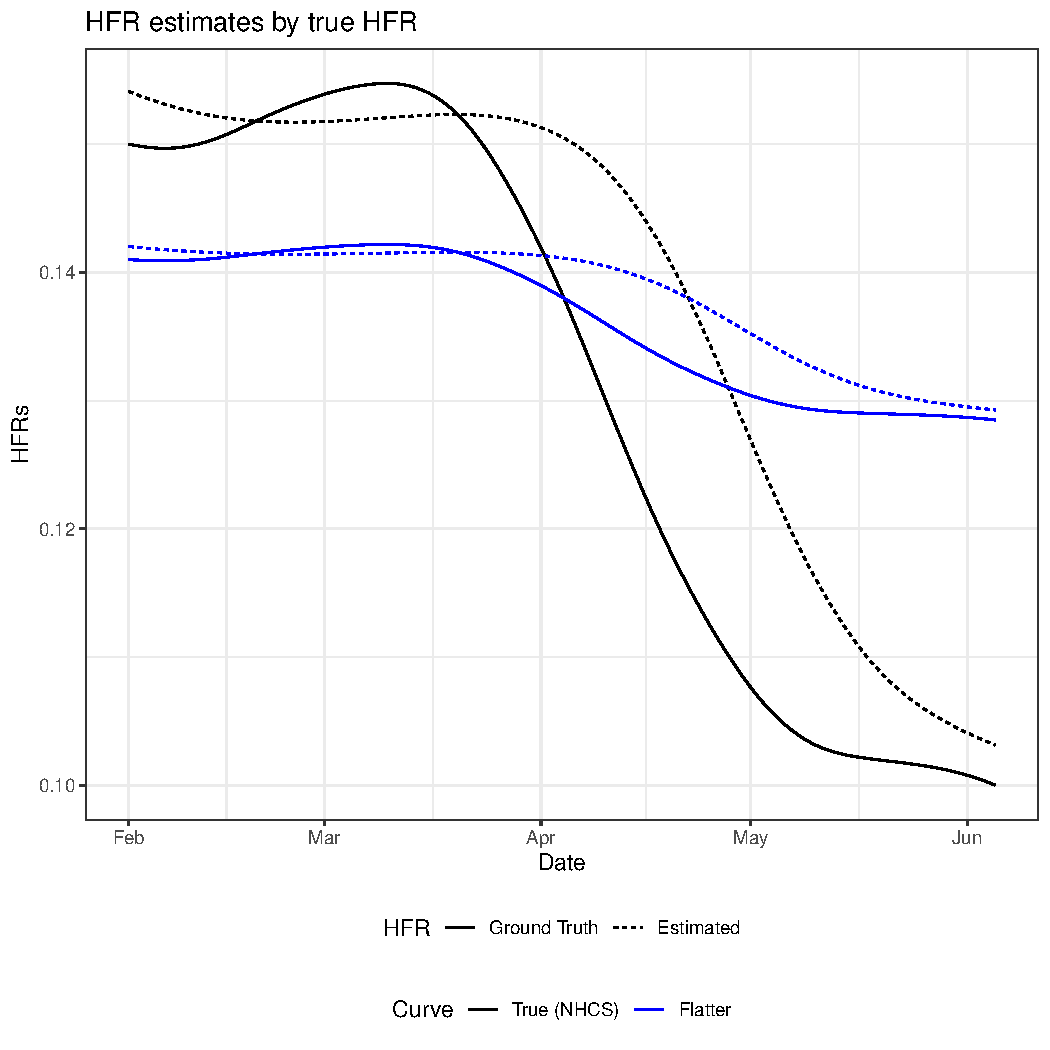
\includegraphics[width=\linewidth]{Figs/Simulated/toy_chging_hfr.pdf}
         \caption{}
         \label{fig:toy_hfr}
     \end{subfigure}
     % \hfill
     \begin{subfigure}[b]{0.32\linewidth}
         \centering
         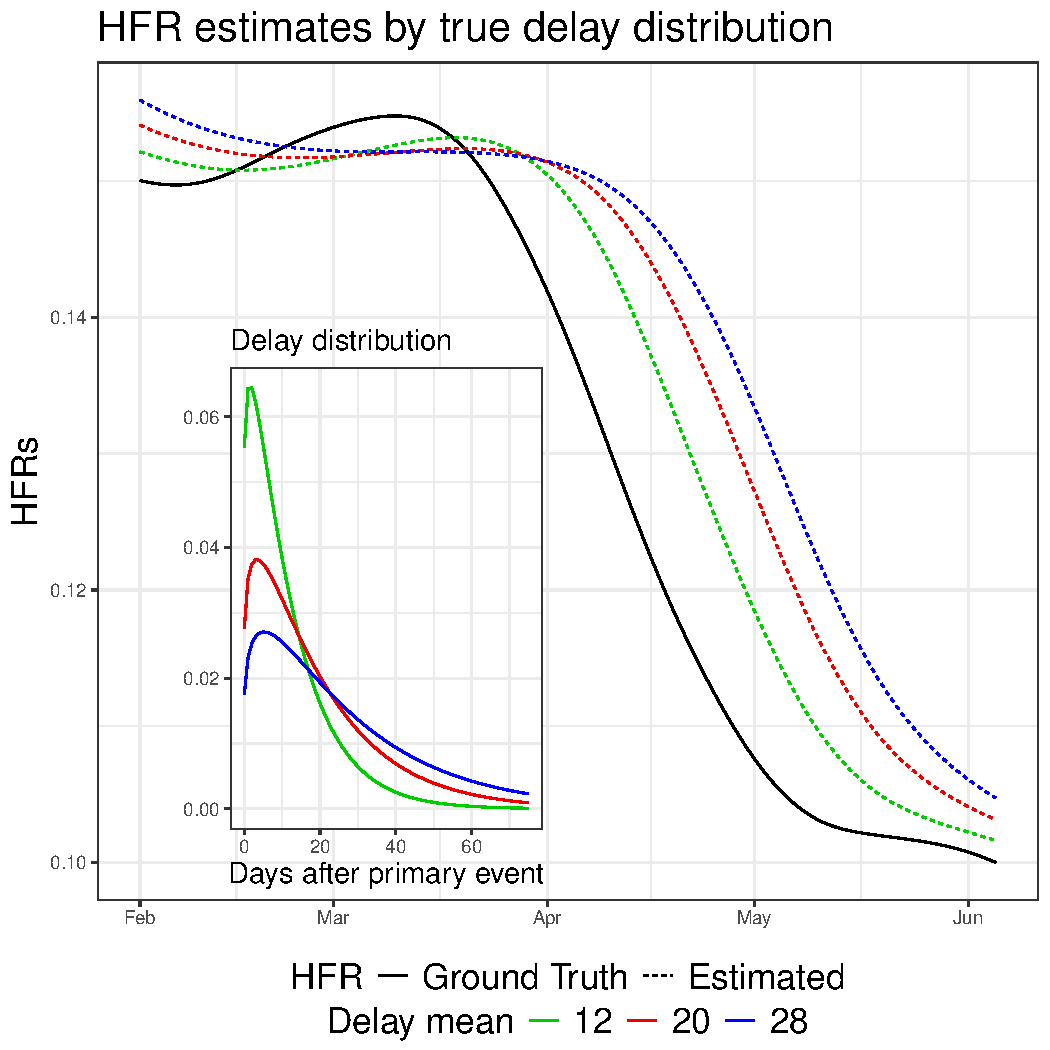
\includegraphics[width=\linewidth]{Figs/Simulated/toy_delay_distr.pdf}
         \caption{}
         \label{fig:toy_delay}
     \end{subfigure}
     % \hfill
     \begin{subfigure}[b]{0.32\linewidth}
         \centering
         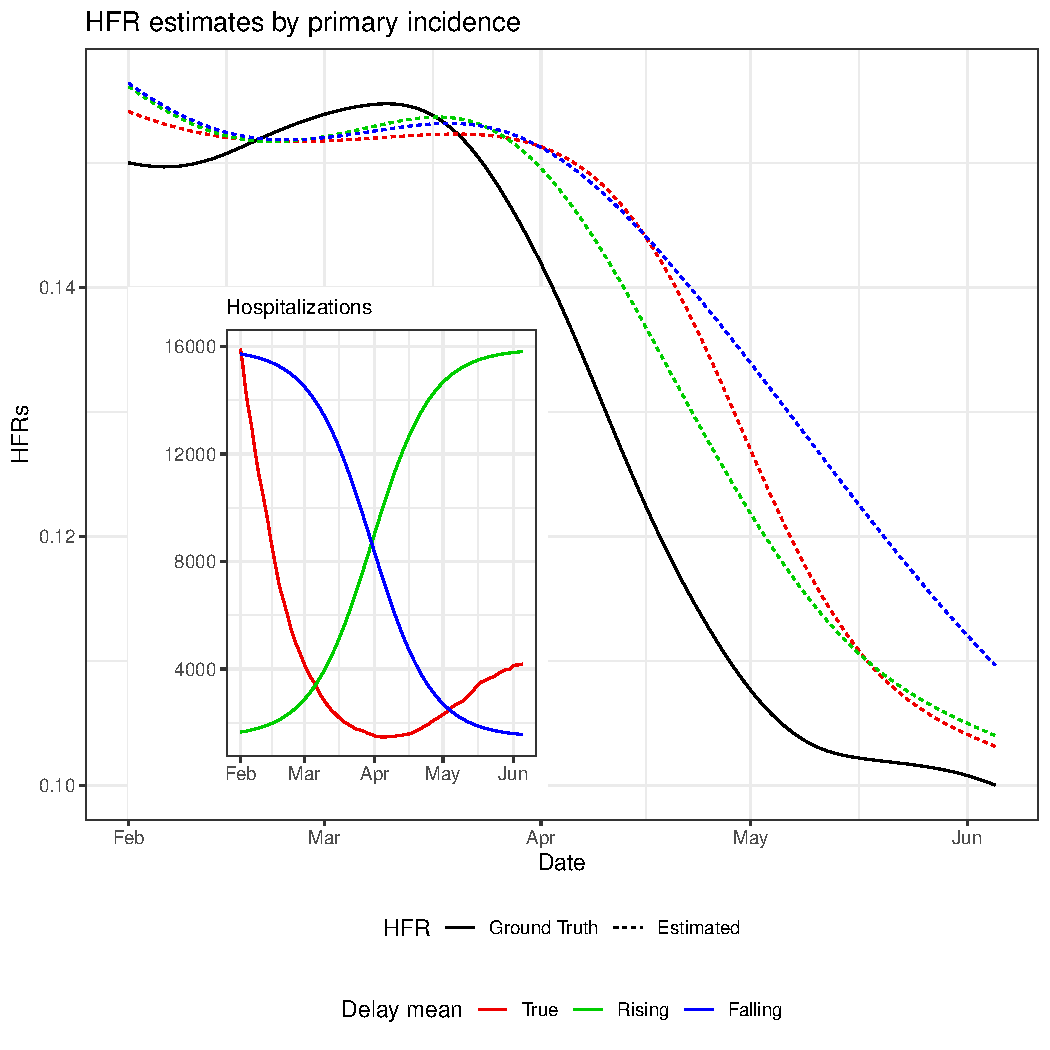
\includegraphics[width=\linewidth]{Figs/Simulated/toy_chging_primary.pdf}
         \caption{}
         \label{fig:toy_primary}
     \end{subfigure}
        \caption{Simple examples of severity rate bias. Deaths computed noiselessly from \eqref{eq:model}, with NCHS HFRs and HHS hospitalizations from early 2022. \ref{fig:toy_hfr} and \ref{fig:toy_primary} use delay distribution fit on JHU deaths (\ref{sec:setup}).}
        \label{fig:bias_ex_main}
\end{figure}


As noted previously, the convolutional ratio is equivalent to the lagged ratio if $\gamma$ is a point mass distribution at $\ell$. In this oracle setting, this indicates all secondary events occur after exactly $\ell$ days, a highly unrealistic situation. Nevertheless, if this is the case, then 

$$\text{Bias}(\hat{p}_t^\ell) = \text{Bias}(\hat{p}_t^\gamma) = p_{t-\ell}-p_t.$$
\noindent This toy setting and others are discussed in Appendix \ref{apx:analysis}.

\subsection{Misspecified analysis}\label{sec:misp}

The above section considered the bias of the convolutional ratio where the true delay distribution $\pi$ is known. We now consider the more general case, in which it is instead replaced with a plug-in estimate $\gamma$. Note the bias of the lagged estimator is a special case, where the plug-in distribution is a point mass at lag time $\ell$. 

\begin{theorem}\label{thm:misp}
Assume the true delay distribution $\pi $ is constant over time, and its maximal length $d$ exceeds that of the plug-in distribution $\gamma$. 
Define $R^\gamma := \frac{\sum_{j=0}^d X_{t-j}\pi_j}{\sum_{j=0}^d X_{t-j}\gamma_j}$, which compares how the delay distributions convolve against the most recent primary incidence levels. The misspecified bias is
% The bias of this misspecified estimator can be expressed additively in terms of the rescaled oracle bias plus a misspecification error term.

\begin{equation}\label{eq:MispBias}
         % \text{Bias}(\hat{p}_t^\gamma = \frac{\sum_{j=0}^d X_{t-j}\pi_j}{\sum_{j=0}^d X_{t-j}\gamma_j}\text{Bias}(\hat{p}_t^\pi) + p_t\big[ \frac{\sum_{k=0}^d X_{t-k}\pi_k}{\sum_{j=0}^d X_{t-j}\gamma_j}-1\big].
          \text{Bias}(\hat{p}_t^\gamma) = R^\gamma\text{Bias}(\hat{p}_t^\pi) + p_t\big[ R^\gamma-1\big].
\end{equation}
\end{theorem}
\ahcomment{
  Comment on notation: should $R^\gamma$ get a subscript-$t$ as well?
}

Theorem \ref{thm:misp}, proven in Appendix \ref{apx:misp_pf}, provides an additive decomposition of the misspecified ratio's bias. One term scales the oracle bias, and the other solely expresses misspecification. Which of these two terms will dominate depends on the true severity rate $p_t$, the oracle bias, and the ratio $R^\gamma$. If oracle bias is small, for example, then its multiplicative scaling should have relatively little effect, in which case the misspecification term may drive bias. In both terms, $R^\gamma$ dictates the extent to which the misspecified distribution alters the bias.
% The extent of the change from the oracle bias depends on the ratio $R^\gamma$. 
% $\text{Bias}(\hat{p}_t^\pi)$. 

Suppose primary events have evened out somewhat after falling for a long time (see April 2022 in Fig. \ref{fig:misspecified}). If the plug-in delay distribution is too light-tailed, then $R^\gamma>1$, since it does not upweight distant dates with high primary counts. Therefore, this distribution inflates the oracle bias multiplicatively and adds positive misspecification bias. If primary events have consistently risen instead, then $R^\gamma < 1$, so the oracle bias term would shrink and the misspecified bias would be negative.
\ahcomment{
  To confirm: if the primary events have consistently risen, then the oracle
  bias term would be negative, right?  And so the misspecification term would
  also be negative, meaning the absolute bias would increase?
}
These relations may be more complicated if primary incidence has changed direction throughout the delay distribution.

\ahcomment{
  I think the bias expression~\eqref{eq:MispBias} is really clear and
  elegant.  Just again thinking through ``worst case'' / ``boundary'' values
  of the bias, assuming that $\pi$ is fixed and we can vary over $\gamma$.
  Just my thoughts... you have thought through all of this yourself already.

  \begin{itemize}
    \item Since $\pi$ is fixed, so is $\sum_{j=0}^{d} X_{t-j}\pi_j$; assume
      it is nonzero.  (If it is zero, then the oracle bias is ill-defined
      anyways.
    \item The denominator ranges between $\min_{j=0,\dotsc,d} X_{t-j}$ and 
      $\max_{j=0,\dotsc,d} X_{t-j}$.  That means that the ability of the
      estimator under misspecification to exhibit ``pathologies'', like having
      $R^\gamma$ close to 0 or infinity, is controlled by the relative scale
      of the primary incidence during the time range $t-d, \dotsc, t$, namely
      how far the minimum and maximum are from the weighted mean of primary
      incidence, as dictated by the oracle distribution $\pi$.  These
      worst case scenarios only happen if we are unlucky enough to have
      a point-mass $\gamma$ that exactly targets the minimum/maximum... which
      does in fact happen for the lagged estimator: the point mass is
      placed at a fixed lag, and as the convolution sweeps across the
      primary incidence curve, there are bound to be times when it picks
      up the minimum/maximum of the primary incidence over its window. 
      Figure~\ref{fig:misspecified} illustrates this perfectly... the ratio
      $R^\gamma$ for the lagged estimator fluctuates away from 1 way more
      than either of the convolutional estimators.
    \item Here's something interesting to note: the bias under misspecification
      can never be smaller than $-p_t$, which is achieved when $R^\gamma=0$.
      Why is this the case?  The oracle bias will never be smaller than
      $-p_t$, because it is a convex combination of $\{p_{t-k}-p_t\}_{k=0}^d$,
      and each of those terms is no less than $-p_t$ because the severity
      rates are positive.  Knowing that, \eqref{eq:MispBias} can be rewritten
      \begin{equation*}
        R^\gamma (\text{Bias}(\hat{p}_t^\pi) - p_t) - p_t,
      \end{equation*}
      where the term $(\text{Bias}(\hat{p}_t^\pi) - p_t)$ is positive.  This
      sanity checks the fact that we never estimate a negative severity rate,
      so the worst-case ``negative'' bias is $-p_t$.  Maybe more interestingly,
      it points out an asymmetry in $\hat p_t$ errors: underestimation of the
      severity rate is bounded below by $-p_t$, but overestimation of the
      severity rate can be unbounded, under misspecification.  (In principle
      one would never estimate $p_t > 1$, so the upper bound would $1-p_t$.)
    \item On the other hand, while the oracle bias also cannot be smaller
      than $-p_t$, it has a sharper upper bound, which is $p_{t-k}-p_t$,
      maximizing over $k=0,\dotsc,d$.
  \end{itemize}
}

% When the plug-in delay distribution hits less mass of the incidence curve - for example, if $\gamma$ is lighter-tailed than $\pi$ and primary events are falling - then $R^\gamma > 1$. 

For the lagged estimator, \ref{thm:misp} simplifies to
\begin{equation}\label{eq:LagBias}
         \text{Bias}(\hat{p}_t^\ell) = \frac{\sum_{j=0}^d X_{t-j}\pi_j}{X_{t-\ell}}\text{Bias}(\hat{p}_t^\pi) + p_t\big[ \frac{\sum_{k=0}^d X_{t-k}\pi_k}{X_{t-\ell}}-1\big].
\end{equation}
In some cases,  $\gamma_k=\mathds{1}\{k=\ell\}$ can be thought as a light-tailed distribution. It assigns all its mass at $\ell$ - chosen to be around the mean of $\pi$ - and none in the long tail of $\pi$. In the flattened-out period around April 2022, the lagged estimator has similar positive bias as the short-tailed convolutional ratio. 

Overall, however, the lagged estimator's bias is more subtle because it relies exclusively on primary incidence $\ell$ days ago. When counts rise sharply between $t-\ell$ and $t$, the ratio $R^\ell>1$ due to its small denominator. In contrast, a smooth, light-tailed choice of $\gamma$ will emphasize recent high counts more than the true distribution $\pi$, so $R^\gamma < 1$. Figure \ref{fig:misspecified} highlights this divergence in behavior as hospitalizations peak in mid-January. 

The lagged estimator also has interesting behavior as primary incidence falls from its peak. The denominator of $R^\ell$ is large, since counts neared the peak $\ell$ days ago. Meanwhile, the numerator is smaller due to its inclusion of lower counts before and after the peak. As a result, $R^\ell<1$, contributing negative bias. Misspecified smooth delay distributions will be less biased under these conditions, since they incorporate the lower counts into the denominator of $R^\gamma$. This explains the lagged ratio's spurious dip in February 2022. 

% Its behavior diverges from the short-tailed ratio as hospitalizations peak in mid-January. Hospitalizations rose sharply to this peak, such that counts were substantially lower just $\ell=20$ days ago. Consequently, the ratio $R^\ell$ surges to 1.5, and the bias spikes upwards. Figure \ref{fig:sims}

% \textcolor{red}{(THIS IS WRONG): \noindent By nature, $\gamma_k=\mathds{1}\{k=\ell\}$ is a light-tailed distribution. It assigns all its mass at $\ell$, and none in the long tail of $\pi$. Consequently, we can generally expect the lagged estimator to have $R^\ell > 1$ when primary events are falling, and $R^\ell<1$ when they are rising. 
% }

\begin{figure}
    \centering
    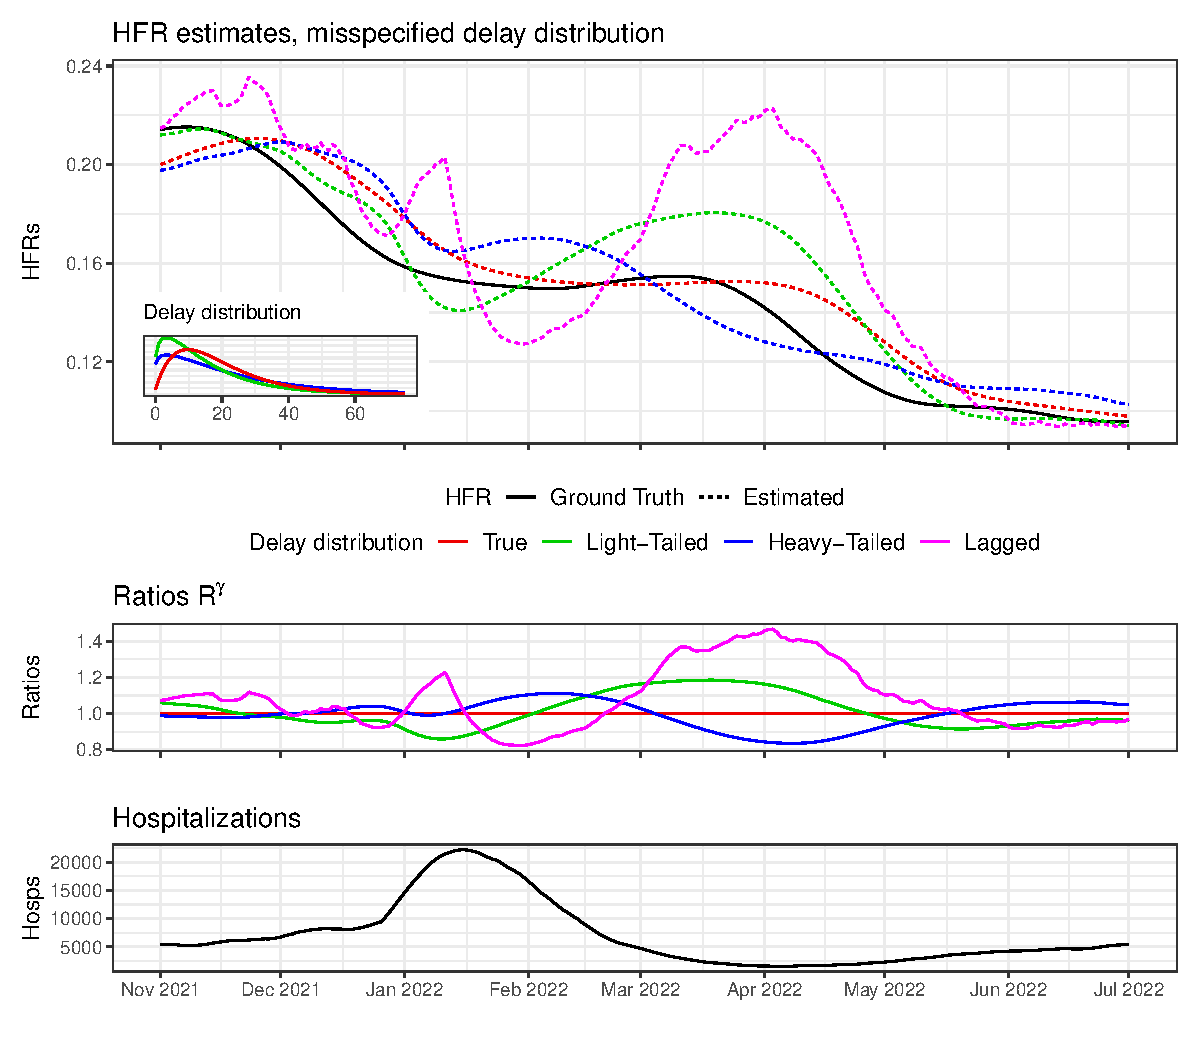
\includegraphics[width=.8\linewidth]{Figs/Simulated/toy_misp.pdf}
    \caption{HFR estimates under misspecification. Convolutional ratio estimates with true delay distribution (mean 20), misshapen gammas (mean 16 and 20), and point mass (i.e. lag) at oracle mean. HHS hospitalizations, NCHS HFRs, and deaths from \eqref{eq:model}.}
    \label{fig:misspecified}
\end{figure}

\ahcomment{
  I really like Figure~\ref{fig:misspecified}... would it be possible to inset
  the distributions onto the top panel?  And label the kernels with their
  means (like in Figure~\ref{fig:toy_hfr}), and you could put a point-mass
  kernel for the lagged estimator (vertical line with a dot on top).  This
  would allow the reader to immediately know what you mean by the different
  delay distributions.
}

% \textcolor{brown}{For...}


\subsection{Experimental setup}\label{sec:setup}
\ahcomment{
  Minor nit: would you consider moving Section~\ref{sec:setup} to
  Section~\ref{sec:analysis}?  Then Section~\ref{sec:methods} would be all
  mathematical description of the estimators, and Section~\ref{sec:results}
  would be all empirical evalution (on real and synthetic data).
}
\subsubsection{HFR estimation}
% Our experiments focus on the Hospitalization-Fatality Rate (HFR) during COVID-19. While this is a less commonly used metric than the Case-Fatality Rate (CFR), the two should exhibit the same statistical biases. Moreover, CFR may slightly misrepresent our analyses because the model relating cases to deaths may be slightly different. Case reporting during COVID suffered significant time delays, with some cases being reported \textit{after} the death. Therefore, the delay distribution for CFR may not have non-negative support. Unlike case data, the Department of Health and Human Services (HHS) reported hospitalizations in real time based on the date they occurred. This makes hospitalizations a more suitable choice of primary event for study. 

Our experiments focus on the Hospitalization-Fatality Rate (HFR) during COVID-19. Hospitalization reporting was much more complete than case reporting throughout the pandemic. Hospitals were mandated to report new daily admissions to the Department of Health and Human Services (HHS) or face penalties \citep{HHS2023}. The time-to-death delay distribution is indeed supported on integers starting at $k=0$, since hospitalizations are aligned by admission date.

% During the pandemic, data sources counted deaths in different ways. John Hopkins University (JHU) provided the definitive resource for real-time death counts, releasing figures daily. However, these counts reflected the times at which deaths were reported to health authorities, not necessarily when they actually happened. In contrast, the National Center for Health Statistics (NCHS) provide weekly totals for deaths aligned by occurrence. Unlike JHU, the NCHS deaths were not available in real time.

To estimate real-time HFRs, we pulled daily hospitalizations and deaths from the \texttt{epidatr} API, developed by the Delphi Group. Like HHS for hospitalizations \citep{HHS2023}, John Hopkins University (JHU) provided the definitive resource for real-time death counts \citep{JHUepidatr}. These counts reflect the times at which deaths were reported to health authorities, not necessarily when they actually happened. Therefore raw JHU death counts are highly volatile due to reporting idiosyncrasies like day-of-week effects and data dumps. As a result, we used a 7-day trailing average of counts. 

The daily aggregates from JHU and HHS were updated over the course of the pandemic. We pulled both the counts available in real time as well as their finalized versions. Often, the most recent date with available counts lagged several days behind the present. To account for this, we estimated HFRs each week, pulling real-time data 6 days after each date. In the rare chance that requested counts still were unavailable, we imputed with the most recently observed date.
% \textbf{TO DO: explain our versioning schema once it's implemented.}

% To estimate real-time HFRs, we use hospitalizations from HHS and deaths from JHU \citep{JHUepidatr}. Data was pulled from the \texttt{epidatr} API, developed by the Delphi Group. Raw JHU death counts exhibit high volatility due to reporting idiosyncrasies like day-of-week effects and data dumps. For that reason, we used a 7-day trailing average of counts. For each dataset, we used the finalized counts, not the versions that would have been available in real time. Doing so would have likely resulted in even more volatile HFR estimates. %We also obtained finalized weekly deaths from NCHS, again smoothing with a spline.

The two ratio estimators (Eq. \eqref{eq:lagged} and \eqref{eq:conv}) require choices of lag and delay distribution. Appendix \ref{apx:robustness} evaluates the robustness of findings against different hyperparameter values. The experiments in Section \ref{sec:results_real} use a lag of 20 days, which maximizes the cross-correlation between hospitalizations and deaths over all time. We let the delay distribution be a discrete gamma, a common choice. We set its mean to this oracle lag, as lags are often chosen to be the mean of the delay distribution. This mean of 20 matches nicely with a UK study (CITE) that finds a median hospitalization-to-death time of 11 days, and a CDC report that 63\% of COVID deaths are reported within 10 days. We set the standard deviation to 18, because the delay distributions fit by the UK study had standard deviations that were roughly 90\% of their means. 


% However, we set the default choice of lag as 19 days. This is motivated by a UK study finding a median hospitalization-to-death time of 11 days, and a CDC report that 63\% of deaths are reported within 10 days. The convolutional ratio uses an estimate of the hospitalization-to-death delay distribution. A common choice is a discrete gamma distribution, whose standard deviation is comparable to its mean. Empirically, we found a mean of 28 days and standard deviation of 21 days minimized the bias.

\subsubsection{Validation data}
While the true HFRs are unknown, there are sound ways to approximate them. One such approach is to use line-list HFRs from the National Hospital Care Survey \citep{NHCS2023}. The NHCS recorded weekly HFRs from inpatient deaths in a representative subset of 601 hospitals across the US. %We smoothed these HFRs with a spline to account for inter-week variability. 
% \ahcomment{
%     % Do you mean ``intra-week variability'' here?  inter-week variability
%     % is what we want to have remain right?
%     % Yes, thanks for the catch!
%     Also --- genuinely curious --- why did we use a spline 
%     rather than just a 7-day moving average?
%     \textcolor{blue}{The NHCS HFRs were reported weekly, and had a fairly high degree of noise.}
% }

HFRs from aggregate hospitalization and death counts are significantly higher than those from NHCS because not all deaths occur in hospitals. A CDC analysis reported the percentage of inpatient deaths every month from 2020 through 2022; roughly 60\% of COVID deaths occurred in hospitals in 2022, down from nearly 70\% in 2021 and 2022. To account for non-inpatient deaths, we divided the NHCS curve by these percentages. Finally, we smoothed the resulting HFRs with a spline. To do so, we used the \texttt{smooth.spline} function in \texttt{R}, which chooses the smoothness hyperparameter with generalized cross validation. % after again smoothing with a spline. 
% NOTE: The more principled thing to do is to divide by proportion of in-patient deaths L days from each timestep, because hospitalizations at t effect deaths after t. But this is more work to explain.

% Let $\eta_t$ be the unscaled, smoothed NHCS HFRs. I'm not sure whether this is forward- or backward-looking; it just says it's the percentage of confirmed COVID-19 hospital encounters with a discharge status of in-hospital death, presented each week. I think this is forward looking? So they look at all hospitalizations for a given week with known discharge status, and calculate the rate that are deaths?

% Number of deaths should be roughly number of hospitalizations * average HFR. So had scaled $\bar Y = \bar X * c \bar\eta \Leftrightarrow c = \frac{\bar Y}{\bar{\eta} \bar X}$. This didn't quite work, though, since the proportion of in-hospital deaths changes over time. That it falls in 2022 indicates there should be a higher scaling rate to the HFRs, for example. 

% Assuming the NHCS HFRs are forward-looking and the lagged model is correct (lol), the number of inpatient deaths $Y_{t+L}^{in}\approx X_t \eta_t$. Let $s_t$ be the proportion of deaths that die in-hospital at $t$ (this is reported in a monthly window surrounding $t$). Then $s_t Y_t \approx Y_t^{in}$. So $Y_{t+L} \approx \frac{X_t \eta_t}{s_{t+L}}$. That is, I can use $\eta_t/s_{t+L}$ as the HFRs, and ultimately rescale as before if needed. 

We considered two other sources for ground truth HFRs, discussed in Appendix \ref{apx:alt_gt}. Unlike NHCS, these HFRs are obtained from aggregate counts, not line-list data. Fortunately, they are fairly consistent with the rescaled NHCS data, bolstering our trust in it. Of course, the NHCS curve is merely an approximation for the ground truth; its values, especially after mid-2022, may be incorrect. Nevertheless, it is a useful aide with which to judge the fidelity of our HFR estimates.
% but entail making worse assumptions. 

\section{Results}\label{sec:results}

\subsection{National COVID data}\label{sec:results_real}

% \begin{figure}
%     \centering
%     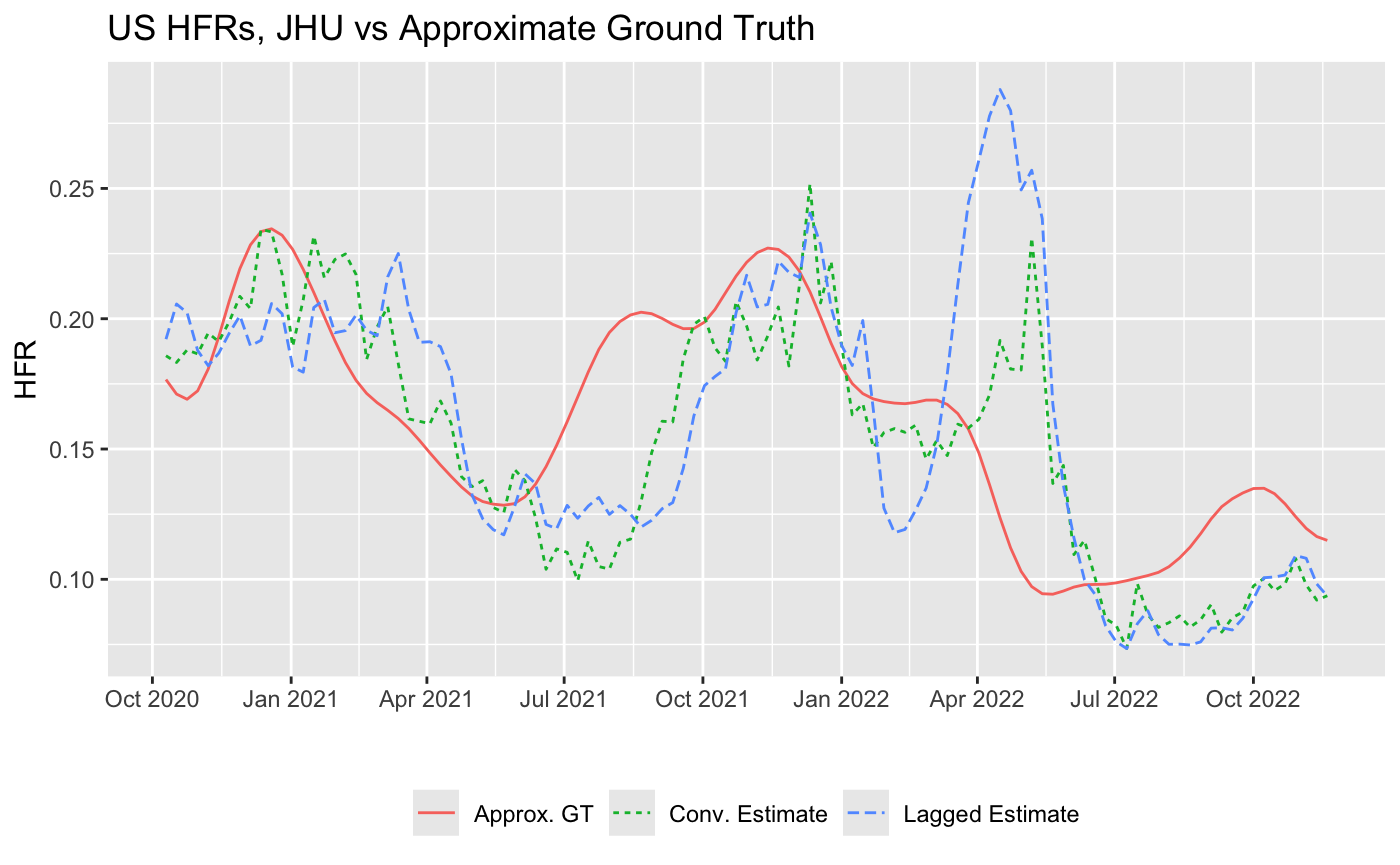
\includegraphics[width=0.8\linewidth]{Figs/Simulated/US_ests_vs_GT.pdf}
%     \caption{Time-varying HFR estimates are highly biased. Terms in both ratio estimates are smoothed over a 7-day window.}
%     \label{fig:basic_est_vs_gt}
% \end{figure}

\begin{figure}
     \centering
     \begin{subfigure}[b]{0.55\linewidth}
         \centering
         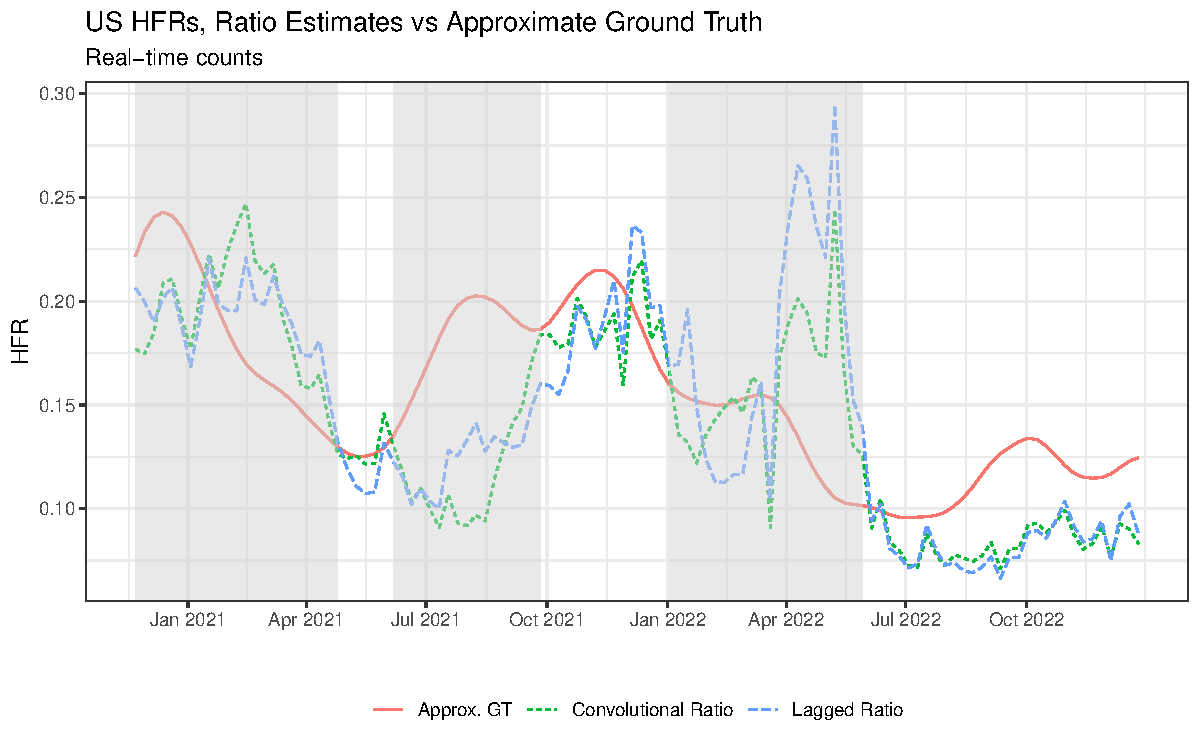
\includegraphics[width=\linewidth]{Figs/Real/US_ests_realtime.pdf}
         \caption{Comparing convolutional and lagged ratios against approximate ground truth. Finalized and real-time counts, Nov. 2020 - Dec 2022.}
         \label{fig:basic_est_vs_gt}
     \end{subfigure}
     \hfill
     \begin{subfigure}[b]{0.4\linewidth}
         \centering
         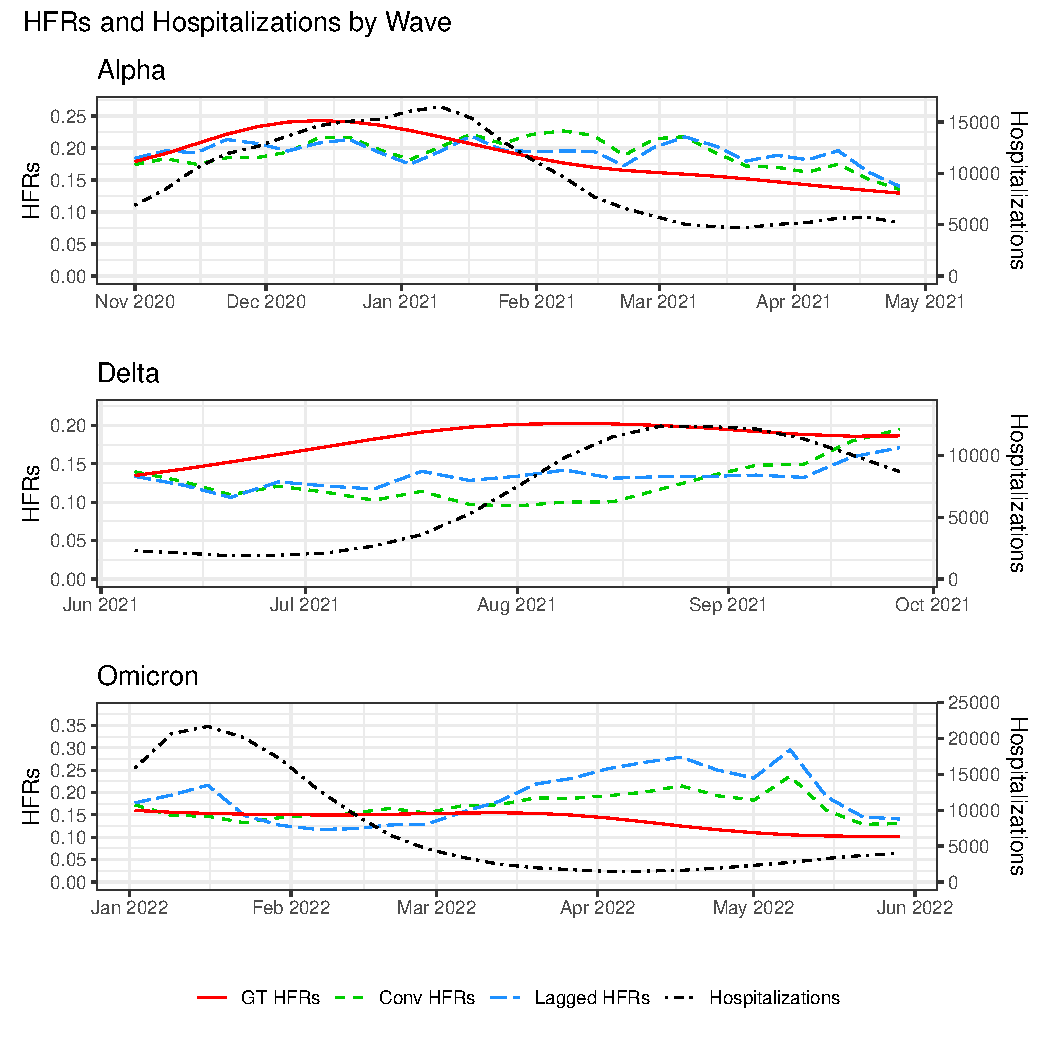
\includegraphics[width=\linewidth]{Figs/Real/hfrs_by_wave.pdf}
         \caption{HFRs and hospitalizations in three periods with major bias.} Finalized counts.
         \label{fig:wave}
     \end{subfigure}
        \caption{Convolutional ratio estimates are biased regardless of which delay distribution is selected.}
        \label{fig:basic_est_vs_gt_figs}
\end{figure}

Figure \ref{fig:basic_est_vs_gt_figs} highlights the bias of these ratio estimators. Both the lagged and convolutional ratios respond very slowly to changes in the HFR. As the HFR declines throughout the Alpha wave in early 2021, both ratios stay around 0.2 for several months. More troublingly, they are very slow to detect the rising HFR in the early Delta period (summer 2021). %A central purpose of these estimators is to inform stakeholders of increased risks in real time; this indicates a failure to do so during the Delta surge.

The most significant bias comes in the middle of the Omicron wave in spring 2022. The true HFRs sharply decline in this period, from a high of roughly 17\% in March to a low of 9\% only two months later. At the same time, the HFR estimates \textit{rise}, peaking over 20\% as the true HFR reaches its nadir. This dramatic surge signals a serious false alarm. 

The well-specified analysis in Section \ref{sec:analysis} explains each of these three failure cases. While this analysis assumes the true delay distribution is known, different choices of delay distribution generally yield the same bias (\ref{apx:robustness}). The convolutional estimator in green may not be far from the oracle ratio, though the lagged ratio has misspecification bias introduced in \ref{sec:misp}. 
\ahcomment{
  Some collected comments:
  \begin{itemize}
    \item Sections should be referred to as, e.g.,
      Appendix~\ref{apx:robustness} and Section~\ref{sec:misp}, to avoid
      ambiguity (reference to figures, etc.).  Refererences that are just a
      number in parentheses should be reserved for numbered equations (and
      referred to using eqref).
    \item For Figure~\ref{fig:basic_est_vs_gt} --- is it necessary to include
      both the results from both the real-time and finalized analyses?
      (I don't know if you and Ryan already discussed this.)  If it's not
      necessary to present both in the main paper (in the same figure), I would
      defer one of them to the Appendix and change the lines from dotted/dashed
      to solid.  That would improve the legibility of the figures
      substantially, and also simplify the legends, etc.  Studying the results
      in Figure~\ref{fig:basic_est_vs_gt}, I don't think that omitting either
      the real-time or finalized results changes the story substantially.
      If only the finalzed counts are being presented in Figure~\ref{fig:wave},
      then maybe just present that in Figure~\ref{fig:basic_est_vs_gt}?
    \item (Especially if Figure~\ref{fig:basic_est_vs_gt} is simplified by
      removing either the finalized or real-time curves), it would be really
      nice to ``shade behind'' in light gray the Alpha, Delta, and Omicron
      waves, so that they can be studied ``in context.''
    \item Would it be possible to explain for each of the panels Alpha,
      Delta, Omicron in Figure~\ref{fig:wave} why the bias is smaller or
      larger for the convolution ratio versus the lagged ratio.  (I think
      a reader/reviewer may ask why, given our toy example showing that
      the lagged estimator generally exhibits larger bias than the convolution
      estimator, by virtue of being more likely to be misspecified, the
      lagged bias is consistently smaller than the convolutional bias for
      Delta.)  We should be able to explain all three based on your analysis
      of the effect of severity rates / primary incidence / delay distribution
      / misspecification on the bias.  If we can explain all three
      convincingly, it would be a very strong empirical illustration (Alpha:
      bias is roughly the same; Delta: convolutional has greater bias;
      Omicron: lagged has greater bias.
  \end{itemize}
}

Firstly, equation \eqref{eq:ConvBias} indicates the bias moves in the opposite direction of the true severity rate. We observe this in the Delta wave, when the HFRs rise well before the ratio estimates do.  
% Rising HFRs result in negative bias, hence the delayed rise in the Delta wave. 
Falling HFRs correspond to positive bias, as observed in early 2021 and 2022. Secondly, the enormity of the bias during Omicron can partially be attributed to the precipitous decline in hospitalizations, as falling primary incidence has been shown to exacerbate the bias. Average daily hospitalizations declined from over 20,000 in mid-January to only 1,500 by April 1. Finally, the delay distribution is relatively long with JHU deaths due to its alignment by report date. This is shown to have a substantial impact on the bias, as analyzed in Appendix \ref{apx:NCHS_deaths}.
% \ahcomment{
% This is great --- I think we would really drive the point home
% if in addition to Figure 1, we had a three-panel figure that
% ``zooms in'' on each of these cases, and specifically labels them
% with each of the three failure modalities, so that the reader
% can see exactly how they correspond to the conditions under
% which bias occurs outlined in Section 2. \textcolor{blue}{How's this look?}%  (Even better if there are toy examples in Section 2, so the reader can see the ``idealized version'' of the failure, and a ``real world'' manifestation of that failure mode.
% }

The misspecified analysis explains central discrepancies between the convolutional and lagged ratios. The lagged estimates dip below the ground truth and convolutional HFRs as hospitalizations fall around February 2022. Shortly thereafter, they spike even higher than the convolutional ratio. These biases both occured in Figure \ref{fig:misspecified}, where deaths were simulated from the same hospitalizations and HFRs. Our analysis attributed the bias to $R^\ell$ in Theorem \ref{thm:misp}, affected by changes in hospitalization counts.

We performed several robustness checks to assess the stability of these findings. Figure \ref{fig:basic_est_vs_gt} compares the convolutional and lagged ratio estimators, finding bias in both. The convolutional estimator is slightly better, but still very problematic. Appendix \ref{apx:robustness} explores the effect of different hyperparameters and locations. By and large, the ratio estimators are biased regardless of these considerations. 

\subsection{Simulated data}


\ahcomment{
  Just to make sure I understand the simulated results properly:
  \begin{itemize}
    \item For both the Short Delay Distribution and the Long Delay
      Distribution, the oracle delay distribution is known to the convolutional
      estimator, and the lagged estimator uses the mean as its lag.
    \item Therefore, these results can be thought of not just as
      ``convolutional versus lagged'' but ``correctly specified versus
      poorly specified'' (poorly specified because it's a point mass kernel,
      even though it has access to the oracle mean).
    \item I don't think it's necessary to include it, but if you wanted to,
      you could add a fourth row to Figure~\ref{fig:sims} with $R^\gamma$
      for the lagged estimator;  I think it is so informative re:
      the additional bias incurred by misspecification, which is the root
      cause of the lagged estimator's exacerbated bias.
  \end{itemize}
}

We further evaluated these methods on simulated deaths whose true HFRs is known. Throughout these experiments, we used observed, finalized HHS hospitalization reports $X_t$, and various models for the HFR and delay distribution. Given a series of time-varying HFRs $p_t$ and delay distribution $\pi$, deaths are defined without noise as according to \eqref{eq:model}

$$Y_t := \sum_{k=0}^d X_{t-k} \mathbb{P}(\text{die at $t$ }\vert\text{ hosp at }t-k) = \sum_{k=0}^d X_{t-k} \pi_k p_{t-k}.$$

To mimic the real data, we first used the same HFRs from NHCS used for validation in \ref{sec:results_real}. We also inverted them and rescaled in order to simulate the opposite trend. Lastly, we explored a stationary HFR of 10\% over all time. The delay distributions were again gamma with standard deviation 0.9 of their mean. We experimented with means of 12 and 24 to illustrate a short and long delay distribution. The ratio estimators used the oracle hyparameters: The true delay distribution for the convolutional ratio, and its mean for the lagged method. Estimates were not smoothed over a trailing window.
% In addition, we used the delay distributions that produced the most reasonable convolutional HFRs on the observed death counts. For NCHS, this was a gamma distribution with mean 11 and standard deviation 10; for JHU, these quantities were 28 and 21, respectively.  (TO DO: replace all this.)

\begin{figure}
    \centering
    % 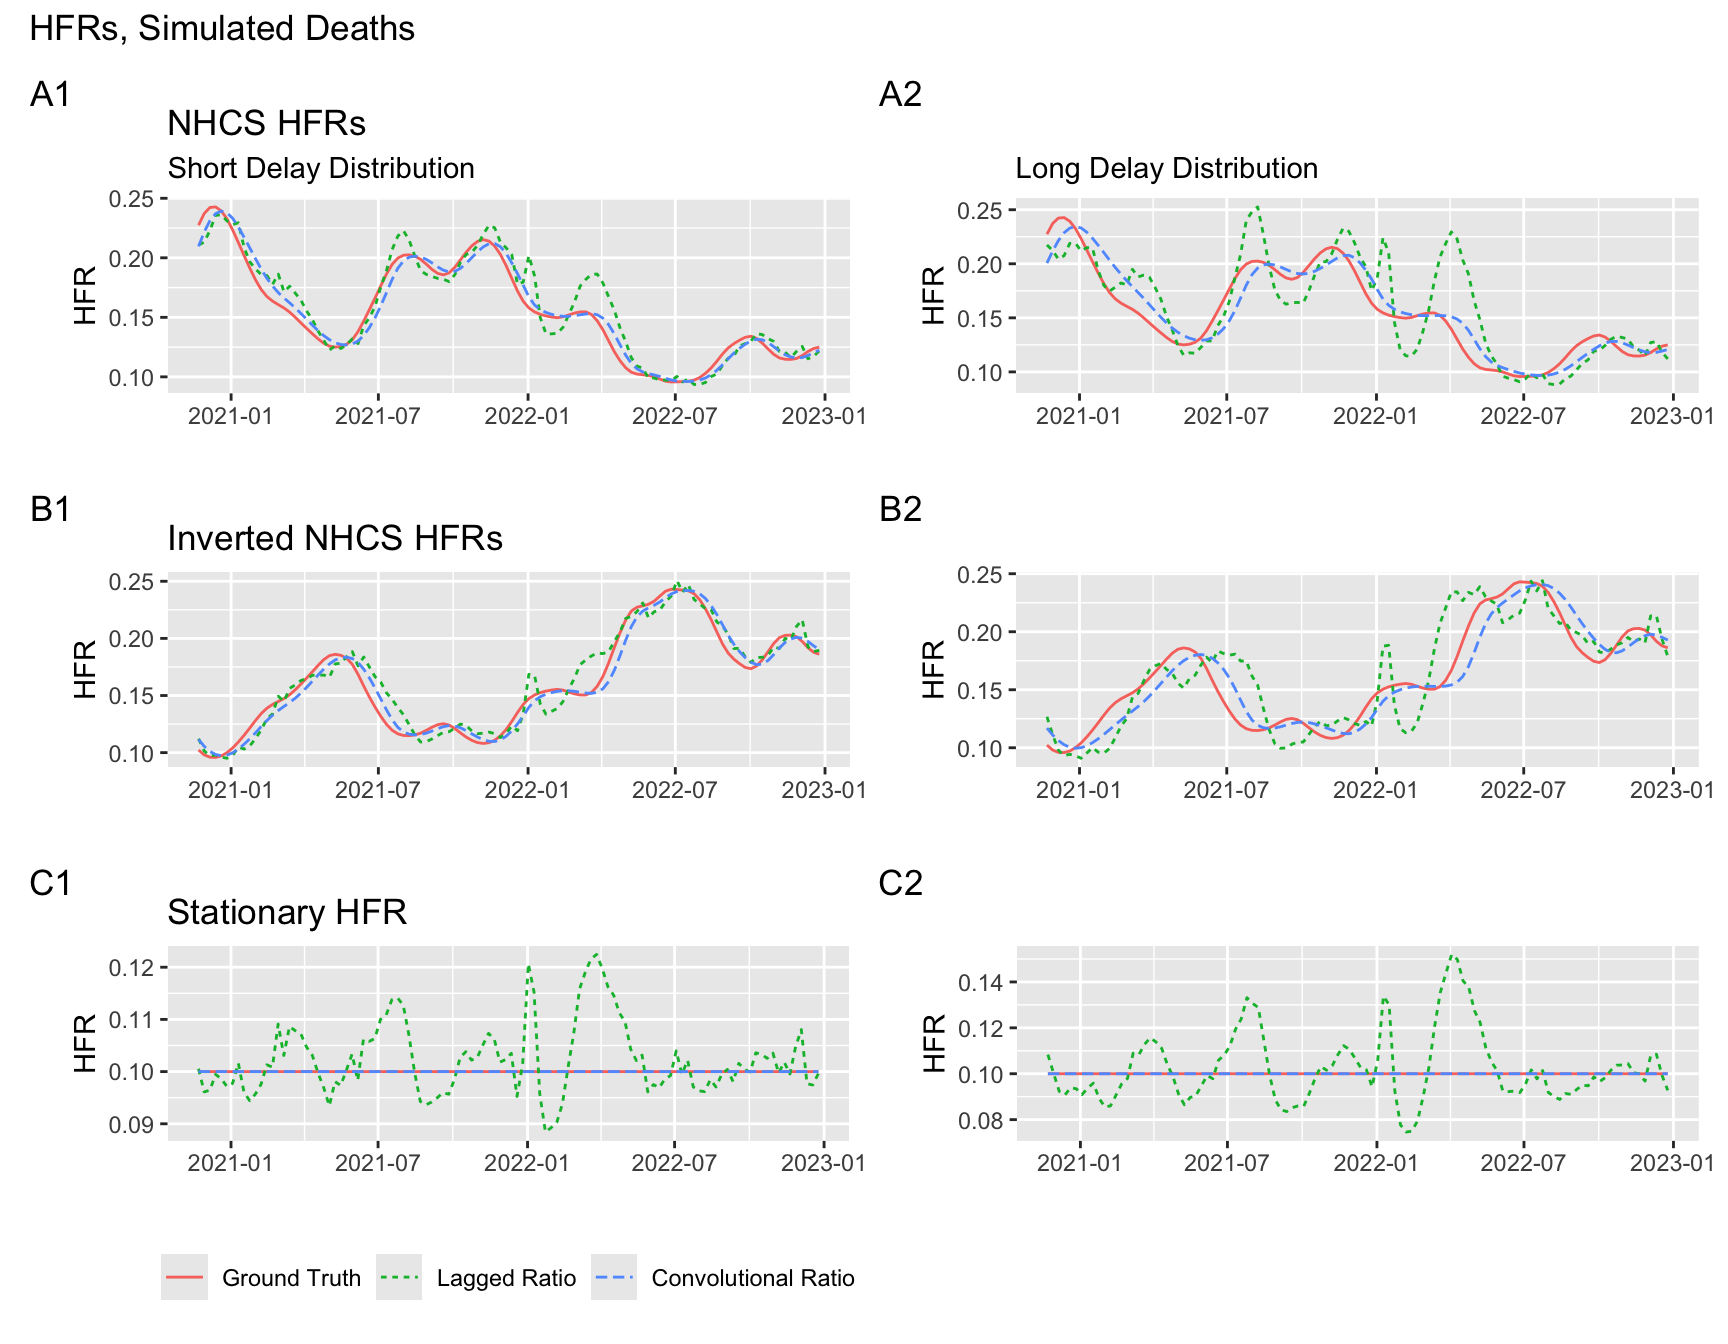
\includegraphics[width=0.9\linewidth]{Figs/Simulated/simulated_results2.pdf}
    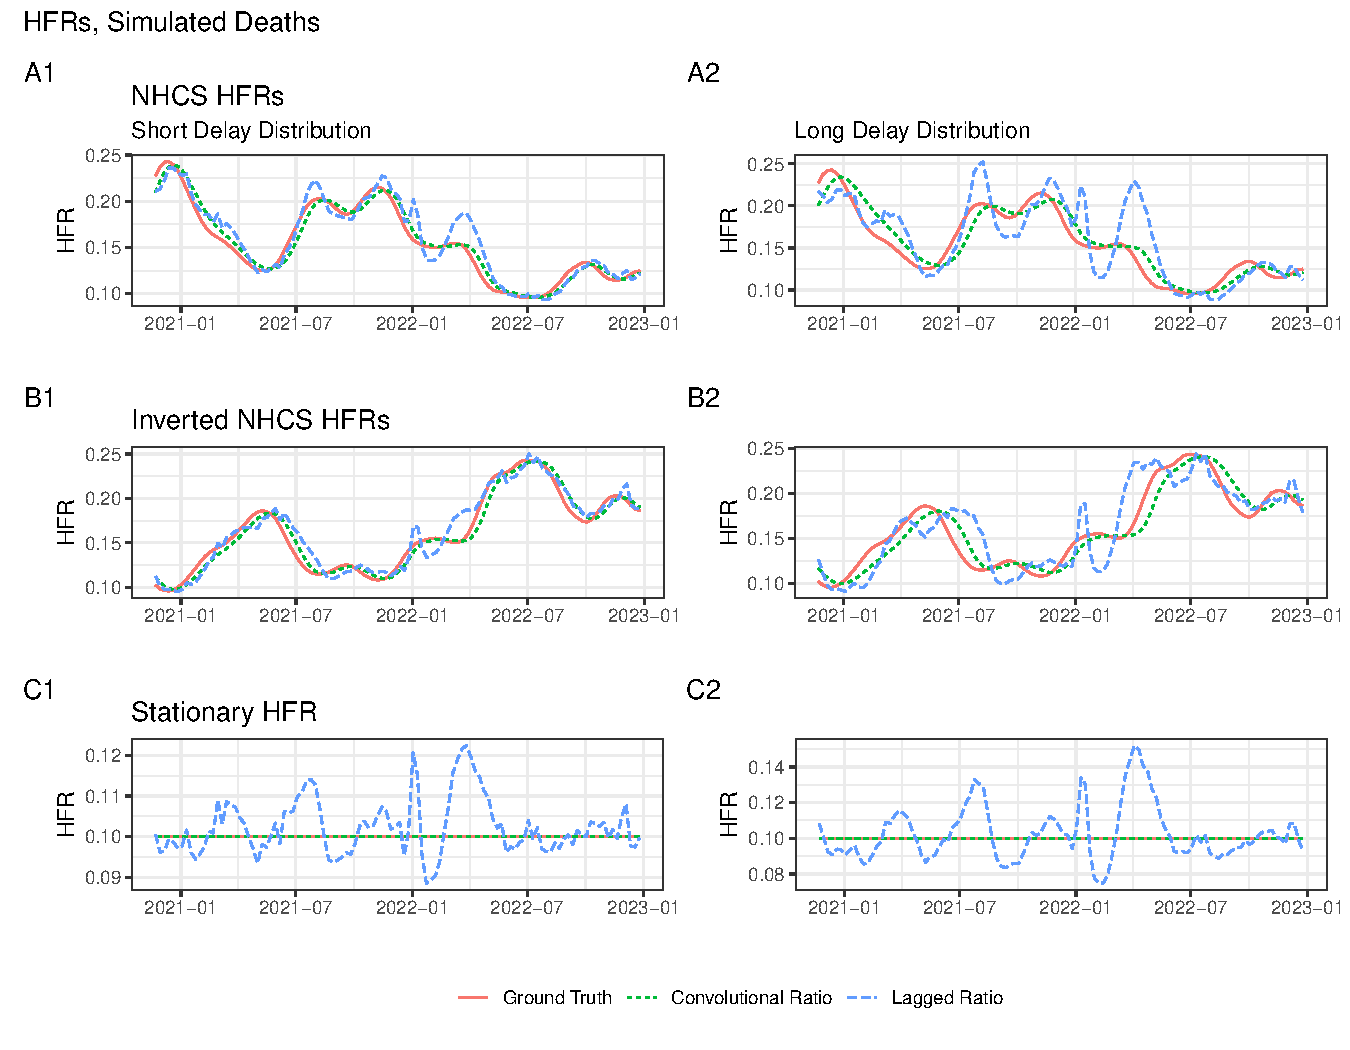
\includegraphics[width=\linewidth]{Figs/Simulated/simulated_results.pdf}
    \caption{True and Estimated HFRs from Simulated Deaths. First column has short delay distribution, second has long.}
    \label{fig:sims}
\end{figure}

Figure \ref{fig:sims} displays the results on the 2 delay distributions and 3 HFR settings. The bias was significantly more pronounced with the longer delay distribution. To assess the relationship between the estimated and true HFRs, we identified the offset that maximized the cross-correlation between the two series. On both the true and inverted NHCS HFRs, this was 7 days for the short distribution, a relatively innocuous gap. However, the offset is 21 days with the longer distribution - concerningly slow during a rapidly changing severity rate like the Delta surge.

Interestingly, the lagged estimator performed considerably worse than the convolutional ratio. When the true HFR changed, the lagged estimates oscillated while the convolutional ratio followed the general trend. In the stationary HFR case, its bias reached as high as 50\%; in contrast, the convolutional estimator was unbiased as anticipated (Eq. \eqref{eq:ConvBias}). This discrepancy is striking, as the lagged ratio is the most commonly-used time-varying estimator. 

Theorem \ref{thm:misp} accounts for this discrepancy. As analyzed in \ref{sec:misp}, the lagged ratio is prone to positive bias as primary incidence has risen sharply. We observe this during the peaks of the Delta and Omicron waves, where the lagged bias spikes even when the underlying HFR is constant. Positive bias is also expected when hospitalizations have leveled out from a decline, which occurs in spring 2022. Lastly, we showed the lagged estimator should have negative bias as primary events fall. This is observed in Delta (September 2021) and Omicron (Februrary 2022). 

\section{Discussion}

Our analyses illustrate that practitioners should take caution when using these time-varying severity ratios. They exhibit considerable bias when severity rates change, particularly the popular lagged ratio. A major purpose of these estimators is to inform stakeholders of changing risks in real time; this bias indicates they may fail to do so in a reliable manner.

Given the drawbacks of these methods, alternative approaches may be preferable when there is reason to believe the true rate is changing. If possible, severity rates can be obtained from line-list data after accounting for right censoring. These rates can then be scaled to a broader population with careful demographic adjustment \citep{verity2020estimates}. 

% Other methods exist to estimate severity rates from aggregate data. 
% When only aggregate data is available, 
More commonly, only aggregate data is available, especially in real time. In that case, other methods may outperform these ratios. \citet{fusedlasso} propose estimating all severity rates at once with a Fused Lasso model, using the relation in Eq. \eqref{eq:model}. Unlike the other approaches, this method is inherently forward-looking, where rates at $t$ are exclusively used to produce secondary events after $t$. However, it may suffer from other sources of bias. It is inclined to estimate smoothly-changing severity rates as piecewise constant, and may yield unstable real-time estimates due to scarce data at the tail.

\citet{UKpaper} also proposed a forward-looking method, this one a ratio between relevant primary and secondary events. However, this method is not applicable in real time, as it uses secondary events after $t$ to compute the severity rate. Nevertheless, it is a useful tool for retrospective estimation. 

Another retrospective tool is aggregate COVID deaths from NCHS, a resource that was not available in real time (Appendix \ref{apx:NCHS_deaths}). Unlike JHU, whose aggregates align deaths by report date, NCHS counts deaths on the day the actually occurred. As a result, the mean of its delay distribution is considerably lower, so it produces more accurate ratio estimates (Fig. \ref{fig:jhu_vs_nchs}, \ref{fig:sims}). Analogously, bias is a more serious issue with earlier primary events. For example, case- or infection-fatality ratios may be more biased than hospitalization-fatality ratios. 

% In a similar vein, deaths from NCHS should be used for retrospective analysis, not JHU. Longer delay distributions have been shown to produce significantly more bias (Fig. \ref{fig:jhu_vs_nchs}, \ref{fig:sims}). Therefore estimates with data that counts secondary events by report date will always be worse. Analogously, bias is a more serious issue with earlier primary events. For example, case- or infection-fatality ratios may be more biased than hospitalization-fatality ratios. 

While still biased, the convolutional ratio generally outperformed the lagged method (Fig. \ref{fig:basic_est_vs_gt}, \ref{fig:sims}). While this estimator is widely used for overall HFRs with cumulative counts, we have not come across any applications for the time-varying case. This further suggests the lagged ratio is overused in practice, though the convolutional ratio may not be the best existing alternative \citep{fusedlasso, UKpaper}.

Severity rates may be biased in ways beyond the statistical bias our work focuses on. Section \ref{sec:setup} mentioned, for example, the fact that estimating HFR from aggregates fails to address the large proportion of deaths occur outside the hospital; \citet{lipsitch2015potential} refer to this as ``survivorship bias." A central challenge for CFR estimation is under-reporting: Not all events are reported, reporting rates change across time, and severe cases are more likely to be reported than mild cases. \citet{reich2012estimating} propose an estimator for a time-invariant \textit{relative} CFR - the ratio of CFRs between groups - that learns these latent reporting rates via the EM algorithm \citep{EM}. \citet{anastasios} applied this in the context of COVID-19, analyzing how the chosen delay distribution affects its results. They also identify other sources of bias, like differences in case definition and testing eligibility.
% TO DO: Discuss other sources of bias in severity rates. e.g. Anastasios, Nick Reich papers.

An interesting connection exists between estimating severity rates and reproduction numbers. A central metric in epidemiology is \textit{case} $R_t$, the average number of secondary infections produced by a single infection at time $t$. Typically estimated in real-time is the closely-related \textit{instantaneous} $R_t$, average number of secondary infections at time $t$ produced by a single primary infection in the past. Comparable to the delay distribution $\pi$ is the renewal equation $g$, which measures the time between primary and secondary infections.

As defined in \eqref{eq:severity}, the severity rate is analogous to case $R_t$. Both concern the average number of secondary events produced by a primary event at time $t$. Moreover, the real-time severity ratios we study are analogous to instantaneous $R_t$, both of which measure how primary events in the past contribute to secondary events at $t$. Indeed, one of the most popular frameworks for estimating instantaneous $R_t$ is strikingly similar to the convolutional ratio \citep{fraser2007,wallinga2007how,cori2013new,rtestim}:
\begin{equation}\label{eq:instRt}
    \hat{R_t} = \frac{I_t}{\sum_{k=0}^d I_{t-k}g_k}.
\end{equation}
% The most fundamental difference between Eq. \eqref{eq:instRt} and \eqref{eq:conv} is the former expresses the rate for a single time series. 
\citet{fraser2007} notes that instantaneous $R_t$ is equal to case $R_t$ if conditions remain unchanged. Similarly, we demonstrated that the convolutional ratio \eqref{eq:conv} is unbiased if the severity rate and delay distribution in the $d$ days before $t$ are stationary. Bias arises as a consequence of changing conditions. Future work could apply this same analytical framework to $R_t$, examining the fidelity of instantaneous $R_t$ as a proxy for case $R_t$. 


\bibliographystyle{apalike}
\bibliography{refs}

\pagebreak
\appendix
\section{Analysis}\label{apx:analysis}
\subsection{Figures}
In this section, we present two examples that further explain the bias. These are more contrived that the ones in \ref{sec:analysis}, for example using unrealistic delay distributions. Nevertheless, their bias can be simplified to simple analytic formulas, isolating the three contributing factors.
% In contrast to the examples in \ref{sec:analysis}, the ones here use contrived delay distributions and

\begin{figure}
     \centering
     \begin{subfigure}[b]{0.45\linewidth}
         \centering
         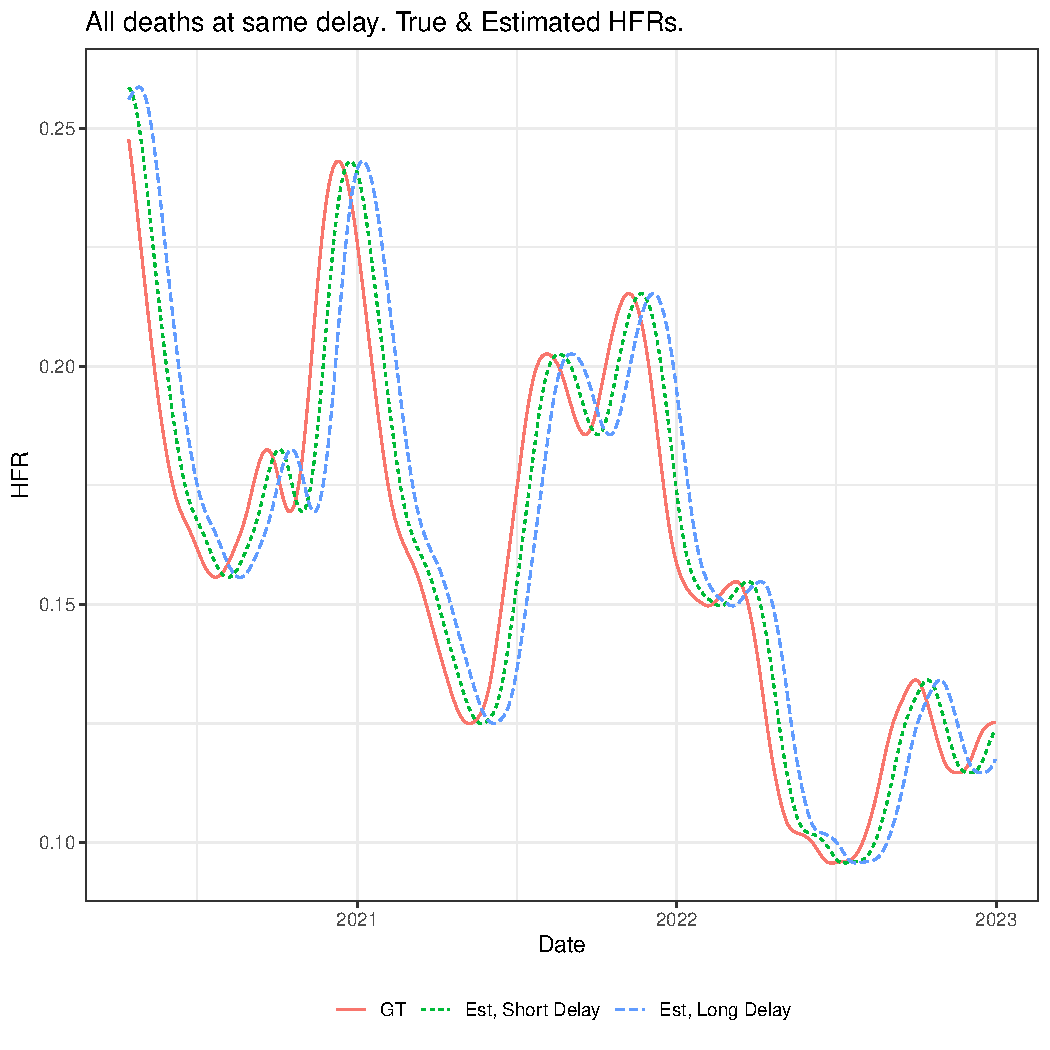
\includegraphics[width=\linewidth]{Figs/Simulated/sim_onehot.pdf}
         \caption{All deaths after $\ell$ days. HFR ratios equivalent; plotting delays of $\ell=14$ and 28 days.}
         \label{fig:onehot}
     \end{subfigure}
     \hfill
     \begin{subfigure}[b]{0.45\linewidth}
         \centering
         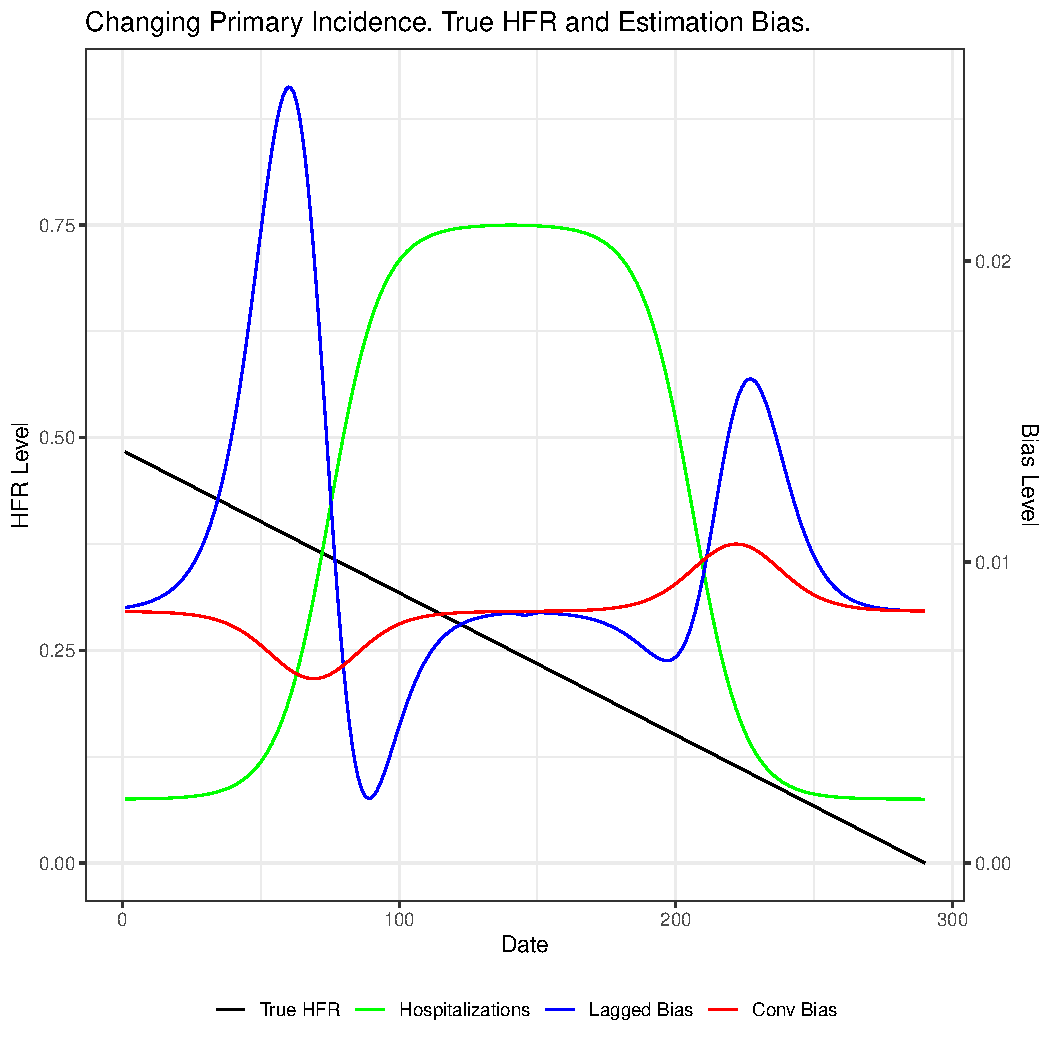
\includegraphics[width=\linewidth]{Figs/Simulated/sim_chging_primary.pdf}
         \caption{Changing primary incidence. Plotting bias of lagged and convolutional ratios.}
         \label{fig:chging_primary}
     \end{subfigure}
        \caption{Toy examples of biased severity rates.}
        \label{fig:bias_ex}
\end{figure}


To elucidate the relationship between changing severity rates and the ratio estimators' bias, consider the trivial case where all secondary events occur after exactly $\ell$ days with no noise. By definition, $\pi_k = \mathds{1}\{k=\ell\}$, so the convolutional and lagged ratios are both $\hat{p}_t = \frac{X_{t-\ell}p_{t-\ell}}{X_{t-\ell}} = p_{t-\ell}$ presuming both have access to the oracle delay distribution. Figure \ref{fig:onehot} displays this with the approximate ground truth HFRs from NHCS. 

In this case, the bias is the change in the true severity rate $p_{t-\ell} - p_t$. The estimator is unbiased only when the severity rate is stationary. Otherwise, for example, the ratio will be 20\% too low if the true severity rate was 20\% lower $\ell$ days ago. 

Intuitively, severity rates may be less similar to the present value $p_t$ further back in time. In this simple example, the bias $p_{t-\ell}-p_t$ is generally larger when $\ell=28$ than $\ell=14$ (Fig \ref{fig:onehot}). This expresses the observation that estimates with heavier-tailed delay distributions tend to have more bias. 

% Constructing another simple case, consider a severity rate that changes monotonically before $t-m$, then is constant until $t$. If the delay distribution assigns all probability mass within the first $m$ days, the convolutional ratio at $t$ will be unbiased. Otherwise, it will be biased, with longer delay distributions producing greater bias. 

Section \ref{sec:analysis} claims that changes in primary incidence levels affect the magnitude of bias for the convolutional ratio. Here, we present simple examples that formalize this claim. First assume primary incidence is constant, in which case the convolutional and lagged ratios are equal. The time series factors neatly out of the bias expression  \eqref{eq:ConvBias}:
$$\text{Bias}(\hat{p}_t^{\gamma}) = \text{Bias}(\hat{p}_t^\ell) = \Big(\sum_{k=0}^d \pi_k p_{t-k}\Big)-p_t.$$
\noindent This is the difference between a weighted average of previous severity rates and the present. Weights for the historical rates are given by the delay distribution, providing further justification for its central role in the bias. 

Next, suppose half of the secondary events occur immediately after the primary event ($t=0$), and the other half after $\ell$ days. Further assume $p_{t-\ell}\neq p_t$, so there is some degree of bias. Then
\begin{align*}
    \lvert\text{Bias}(\hat{p}_t^{\gamma})\rvert &= \frac{\frac{1}{2}\big\lvert X_{t}(p_t-p_t) + X_{t-\ell}(p_{t-\ell}-p_t)\big\rvert}{\frac{1}{2}(X_{t}+X_{t-\ell})} \\
    &=\frac{X_{t-\ell}\lvert p_{t-\ell}-p_t\rvert}{X_{t-\ell}(1+\frac{X_{t}}{X_{t-\ell}})} = \frac{\lvert p_{t-\ell}-p_t \rvert}{1+\frac{X_{t}}{X_{t-\ell}}}
\end{align*}

The absolute bias is monotonically decreasing in $\frac{X_{t}}{X_{t-\ell}}$, the proportion change in primary incidence. Rising primary incidence ($\frac{X_{t}}{X_{t-\ell}}>1)$ yields less bias, while falling levels yield more.

Figure \ref{fig:chging_primary} displays this setting. Hospitalizations are defined as $X = \sigma(s)*9000+1000$, where $\sigma$ is the sigmoid function and $s$ takes 300 evenly spaced steps from -9 to 7. The true HFRs fall from 0.5 to 0 over the same number of even steps. Indeed, the convolutional ratio's bias dips as hospitalizations rise, and rises as they fall. 

When daily hospitalizations approach a constant level, the two estimators become the same ratio, so their biases converge. During periods of change, however, the lagged estimator has different bias. It oscillates up and down, reaching higher bias than the convolutional ratio. 

TO DO: ANALYZE WHY THIS HAPPENS.

\subsection{Misspecification Proof}\label{apx:misp_pf}

The additive bias term is
\begin{align*}%\label{eq:MispBias}
    \text{Bias}(\hat{p}_t) &= \frac{E[Y_t]}{\sum_{k=0}^d X_{t-k}\gamma_k} - p_t \\
    &= \frac{\sum_{k=0}^d X_{t-k}\pi_k p_{t-k}}{\sum_{k=0}^d X_{t-k}\gamma_k} - \frac{\sum_{k=0}^d X_{t-k}\gamma_k p_t}{\sum_{k=0}^d X_{t-k}\gamma_k} \\
    &= \sum_{k=0}^d \frac{X_{t-k}}{\sum_{j=0}^d X_{t-j}\gamma_j}(\pi_k p_{t-k}-\gamma_k p_t) \\
    &= \sum_{k=0}^d \frac{X_{t-k}}{\sum_{j=0}^d X_{t-j}\gamma_k}(\pi_k p_{t-k}-(\pi_k +(\gamma_k-\pi_k)) p_t) \\
     &= \frac{\sum_{j=0}^d X_{t-j}\pi_j}{\sum_{j=0}^d X_{t-j}\gamma_j}\sum_{k=0}^d \frac{X_{t-k}\pi_k}{\sum_{j=0}^d X_{t-j}\pi_j}(p_{t-k}-p_t) -\\
     &\qquad\qquad p_t\sum_{k=0}^d \frac{X_{t-k}}{\sum_{j=0}^d X_{t-j}\gamma_j}(\gamma_k -\pi_k)  \\
     &= \frac{\sum_{j=0}^d X_{t-j}\pi_j}{\sum_{j=0}^d X_{t-j}\gamma_j}\text{Bias}(\hat{p}_t^\pi) + p_t\Big[ \frac{\sum_{k=0}^d X_{t-k}\pi_k}{\sum_{j=0}^d X_{t-j}\gamma_j}-1\Big]
\end{align*}
          % &= \frac{\sum_{j=0}^d X_{t-j}\pi_j}{\sum_{j=0}^d X_{t-j}\gamma_j}\Big[\text{Bias}(\hat{p}_t^\pi) + p_t\sum_{k=0}^d \frac{X_{t-k}\pi_k}{\sum_{j=0}^d X_{t-j}\pi_j}(\frac{\gamma_k}{\pi_k} -1)\Big] \\
          %   &= \frac{\sum_{j=0}^d X_{t-j}\pi_j}{\sum_{j=0}^d X_{t-j}\gamma_j}\Big[\text{Bias}(\hat{p}_t^\pi) + p_t\big[\sum_{k=0}^d \frac{X_{t-k}\gamma_k}{\sum_{j=0}^d X_{t-j}\pi_j}-1\big]\Big]

Alternatively, the bias can be written in a multiplicative form. Modifying the third line yields
\begin{align}
        \text{Bias}(\hat{p}_t^\gamma) &= \sum_{k=0}^d \frac{X_{t-k}}{\sum_{j=0}^d X_{t-j}\gamma_j}(\pi_k p_{t-k}-\gamma_k p_t)\nonumber \\
        &= \sum_{k=0}^d \frac{X_{t-k}\gamma_k}{\sum_{j=0}^d X_{t-j}\gamma_j}(\frac{\pi_k}{\gamma_k} p_{t-k}- p_t).
\end{align}
Interestingly, this means that when if $p_{t-k} < p_t$ and $\gamma_k < \pi_k$, then the $k$\textsuperscript{th} pointwise term here may have smaller bias than in the oracle case. The same holds conversely, with $p_{t-k} > p_t$ and $\gamma_k > \pi_k$. But since $\gamma_k$ is constrained to sum to 1, it’s not clear that it can be systematically chosen to achieve lower bias than $\pi$.

For the lagged estimator, the additive bias is

\begin{align*}
         \text{Bias}(\hat{p}_t^\gamma) &=  \frac{\sum_{j=0}^d X_{t-j}\pi_j}{X_{t-\ell}}\Big[\text{Bias}(\hat{p}_t^\pi) + p_t\sum_{k=0}^d \frac{X_{t-k}}{\sum_{j=0}^d X_{t-j}\pi_j}(\gamma_k -\pi_k)\Big]
\end{align*}


\section{Alternative data sources}
\subsection{Retrospective deaths}\label{apx:NCHS_deaths}

JHU presented daily deaths in real time, aligned by the date they were reported. In contrast, the National Center for Health Statistics (NCHS) provided weekly totals for deaths aligned by occurrence, and were not available in real time. Thus, delay distributions with NCHS deaths have a lighter tail. 

Figure \ref{fig:jhu_vs_nchs} shows this minor change has a significant effect on the bias. It compares the real-time lagged ratios (Eq. \eqref{eq:lagged}) with deaths sourced from JHU and NCHS. JHU is much more biased during the Alpha, Delta, and Omicron periods discussed. For example, NCHS only rises from 12\% to 14\% as Omicron falls, far below JHU's surge above 25\%. As analyzed in \ref{sec:analysis}, JHU's heavier-tailed delay distribution inflates the influence of dates with higher HFRs than the present.

% The shape of the delay distribution plays a significant role in the bias. 

\begin{figure}
    \centering
    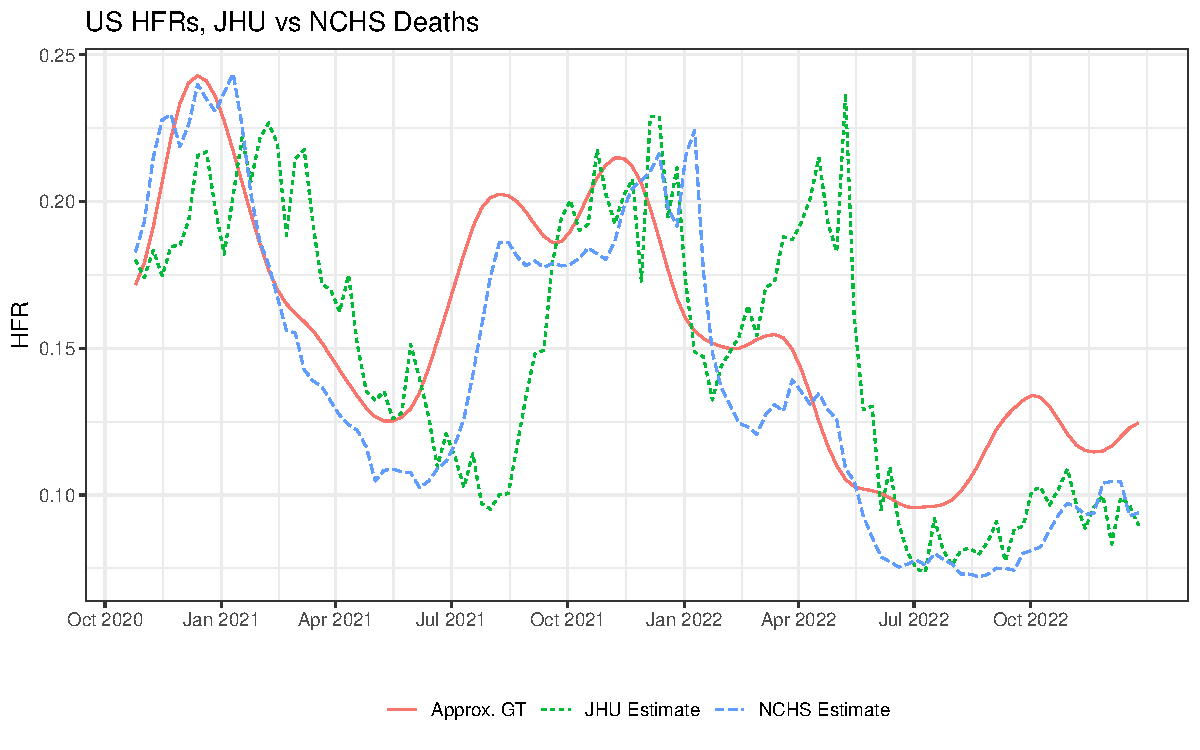
\includegraphics[width=0.7\linewidth]{Figs/Real/jhu_vs_nchs.pdf}
    \caption{Real-time Lagged Ratios, JHU vs NCHS deaths. Seven-day smoothing with 19- and 11-day lags, respectively.}
    \label{fig:jhu_vs_nchs}
\end{figure}


\subsection{Alternative ground truth}\label{apx:alt_gt}

\begin{figure}
    \centering
    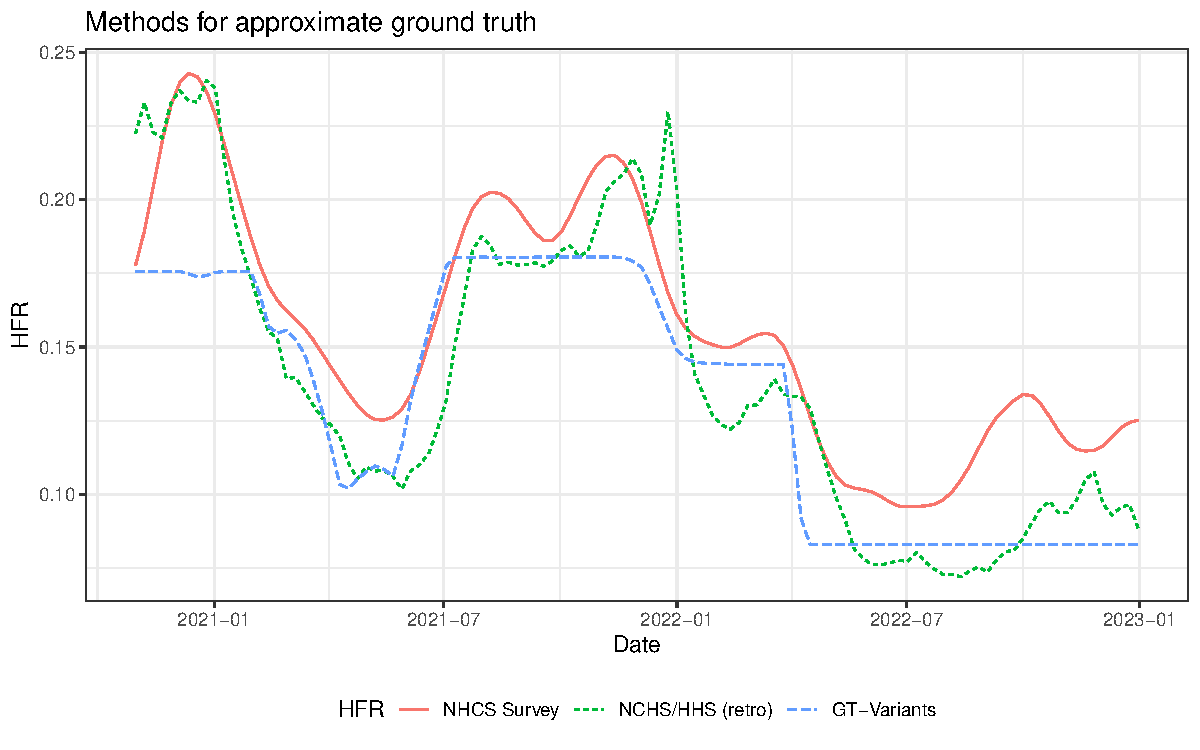
\includegraphics[width=0.8\linewidth]{Figs/Real/ApproxGT.pdf}
    \caption{Methods for Retrospective Ground Truth HFRs.}
    \label{fig:approxGT}
\end{figure}

We considered two retrospective approaches to approximate the ground truth national HFRs over time. The first approach took lagged ratios with aggregate deaths from NCHS. NCHS is a better resource than JHU because it uses death counts from the date they actually occurred, not merely reported. In addition, we take a forward-looking ratio, which is retrospective insofar as it uses data after time $t$ to estimate the HFR.
% Unlike the real-time estimates, we  method is forward-looking and . 

\begin{equation}\label{eq:LaggedRetro}
    \hat{p}_t^{\text{LaggedRetro}} = \frac{Y_{t+L}}{X_t}
\end{equation}
% \noindent Equation \eqref{eq:LaggedRetro} is retrospective because it uses data after time $t$, and therefore is not applicable in real-time. 

The second approach computed a single HFR for each major variant, then mixing by the proportions of variants in circulation. Formally, let $\hat{p}_j$ approximate the HFR of variant $j$; let $v_t^j$ be its proportion of cases at time $t$, where $\sum_j v_t^j = 1 \; \forall t$. The HFR estimate is

$$\hat{p}_t^{\text{Var}} = \sum_j v_t^j \hat{p}_j.$$

Each variant's HFR $\hat p_j$ was defined as the ratio of total NCHS deaths and HHS hospitalizations during the period where it accounted for over 50\% of activate cases. The case proportions $v_t^j$ were obtained from \texttt{covariants.org}. To ensure estimates were reasonable, we only considered the 4 largest variants: The original strain, Alpha, Delta, and Omicron. Because Omicron began with an enormous surge that quickly subsided, we split it into early and late periods at April 1, 2022, following \citep{adjei2022mortality}.

Figure \ref{fig:approxGT} displays the three curves approximating the true HFRs. They have nontrivial differences in magnitude, but move more or less in conjunction. To validate our results, we primarily used the rescaled NHCS HFRs as the least problematic of the three. The retrospective NCHS ratios are subject to statistical bias, expressed in \eqref{eq:LagBias}. The variant-based HFRs are flatter, as they do not account for other sources of variability. Therefore, they do not explain for the statistical bias within each variant period, which arises due to changes in the underlying severity rate.  %unreasonably flat

\section{Robustness checks}\label{apx:robustness}
\subsection{Hyperparameters}
In this section we demonstrate the robustness of our findings against choices of hyperparameters. (All results are with the finalized version of JHU deaths.) First, Figure \ref{fig:window} plots performance over choices of window size parameter. We analyze smoothed versions of the lagged estimator

\begin{equation}\label{eq:laggedSmooth}
    \hat{p}_t^{\ell, W} = \frac{\sum_{s=t-w+1}^{t} Y_s}{\sum_{s=t-w+1}^{t} X_{s-\ell}},
\end{equation}
\noindent as well as the convolutional estimator
\begin{equation}\label{eq:convSmooth}
    \hat{p}_t^{\gamma, W} = \frac{\sum_{s=t-w+1}^{t} Y_s}{\sum_{s=t-w+1}^{t} \sum_{k=0}^d X_{s-\ell-k}\gamma_k}.
\end{equation}

\noindent Results are very similar, indicating the bias does not disappear when smoothing over a longer history. 

\begin{figure}
    \centering
    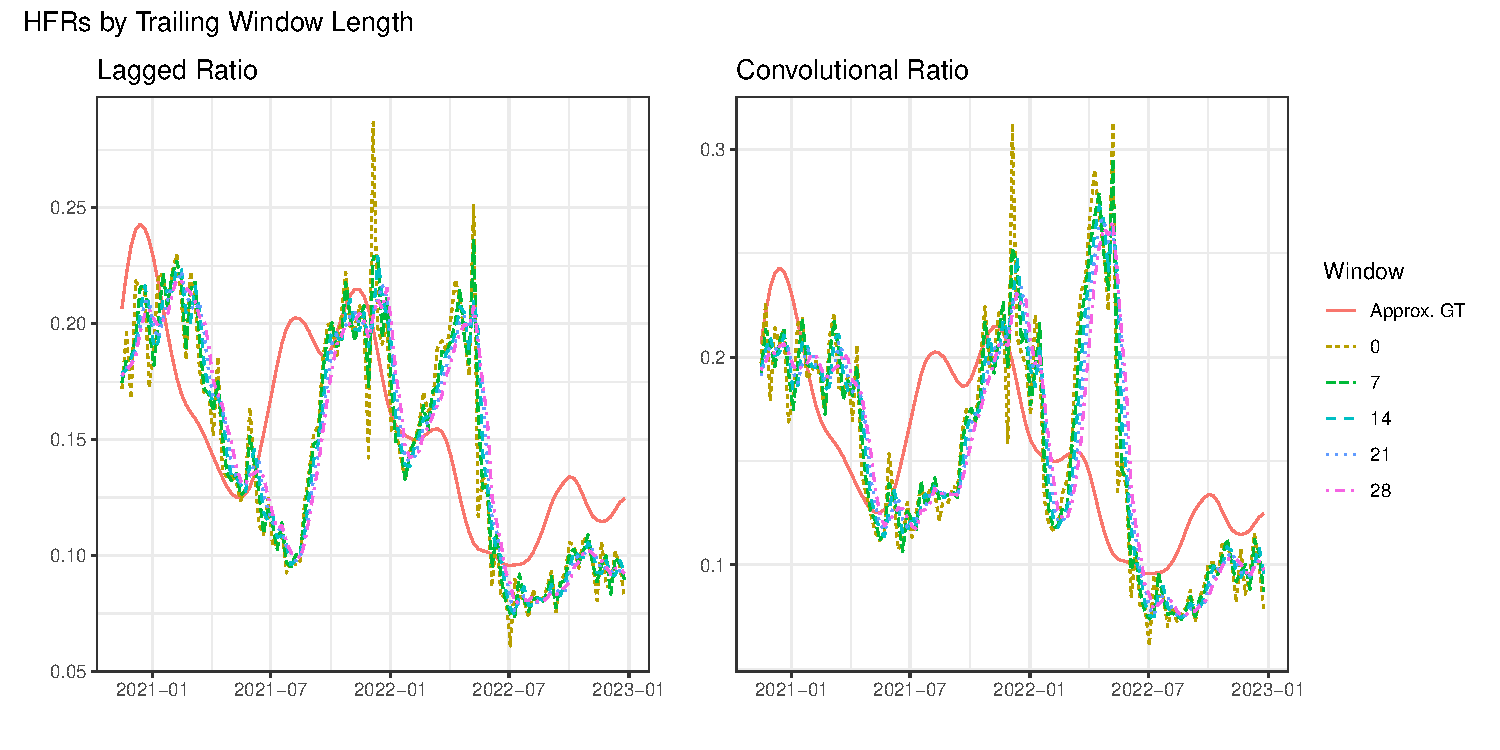
\includegraphics[width=0.75\linewidth]{Figs/Real/window_size.pdf}
    \caption{The length of the trailing window bears little impact on the findings.}
    \label{fig:window}
\end{figure}

We next examine the time-to-death hyperparameters: The lag $\ell$ for the lagged ratio and delay distribution $\pi$ for the convolutional ratio. Figure \ref{fig:lag} displays HFR estimates with lags ranging from 2 to 5 weeks. Unlike the window size, changing this parameter leads to different behavior across lags. Some choices are better than others; a 28-day lag, for example, falls appropriately during Alpha and rises less slowly during Alpha. However, all are biased to varying degrees, most notably the huge spurious surge in spring 2022.

\begin{figure}
    \centering
    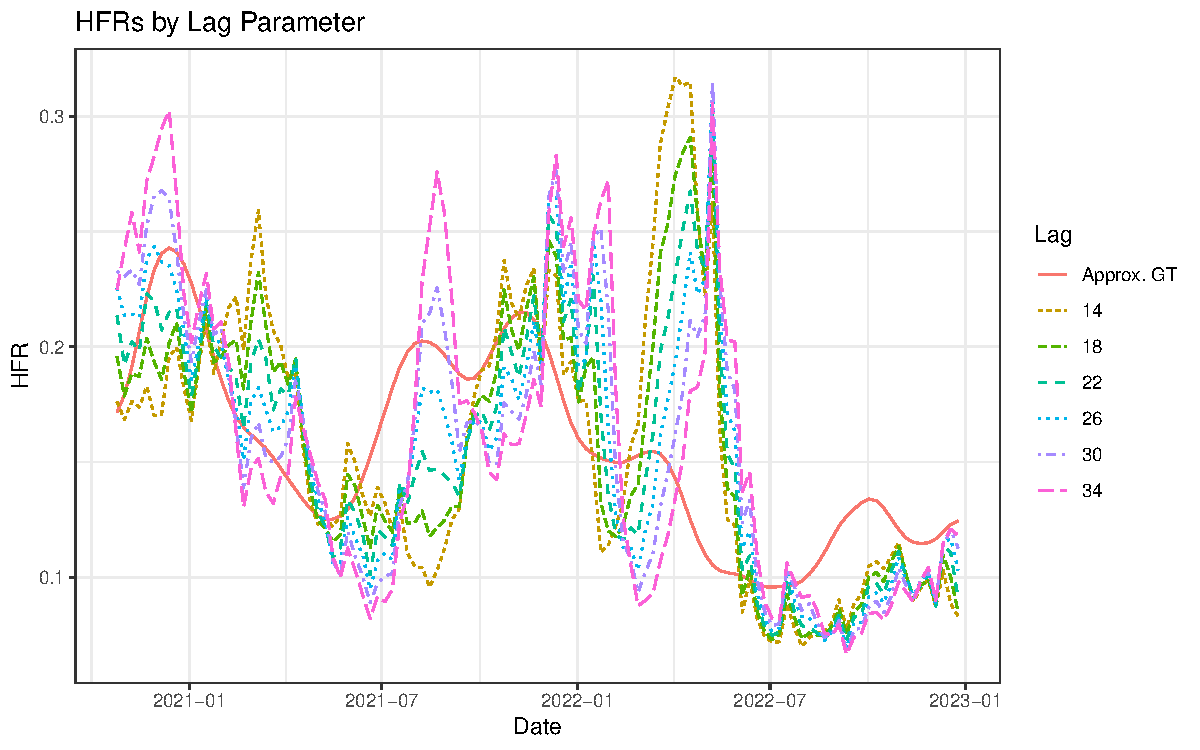
\includegraphics[width=0.7\linewidth]{Figs/Real/hfrs_by_lag.pdf}
    \caption{HFRs are biased regardless of what lag parameter is selected.}
    \label{fig:lag}
\end{figure}

% TO DO: Different delay distribution
Figure \ref{fig:delays} compares the performance of the convolutional ratio across different choices of delay distribution. We kept the discrete gamma shape for each, but varied the mean and standard deviation. As before, Figure \ref{fig:delay1} kept the standard deviation to 90\% of the mean, per \citet{UKdelay}. We also evaluated with a more compact delay distribution in \ref{fig:delay2}. 

% \begin{figure}
%     \centering
%     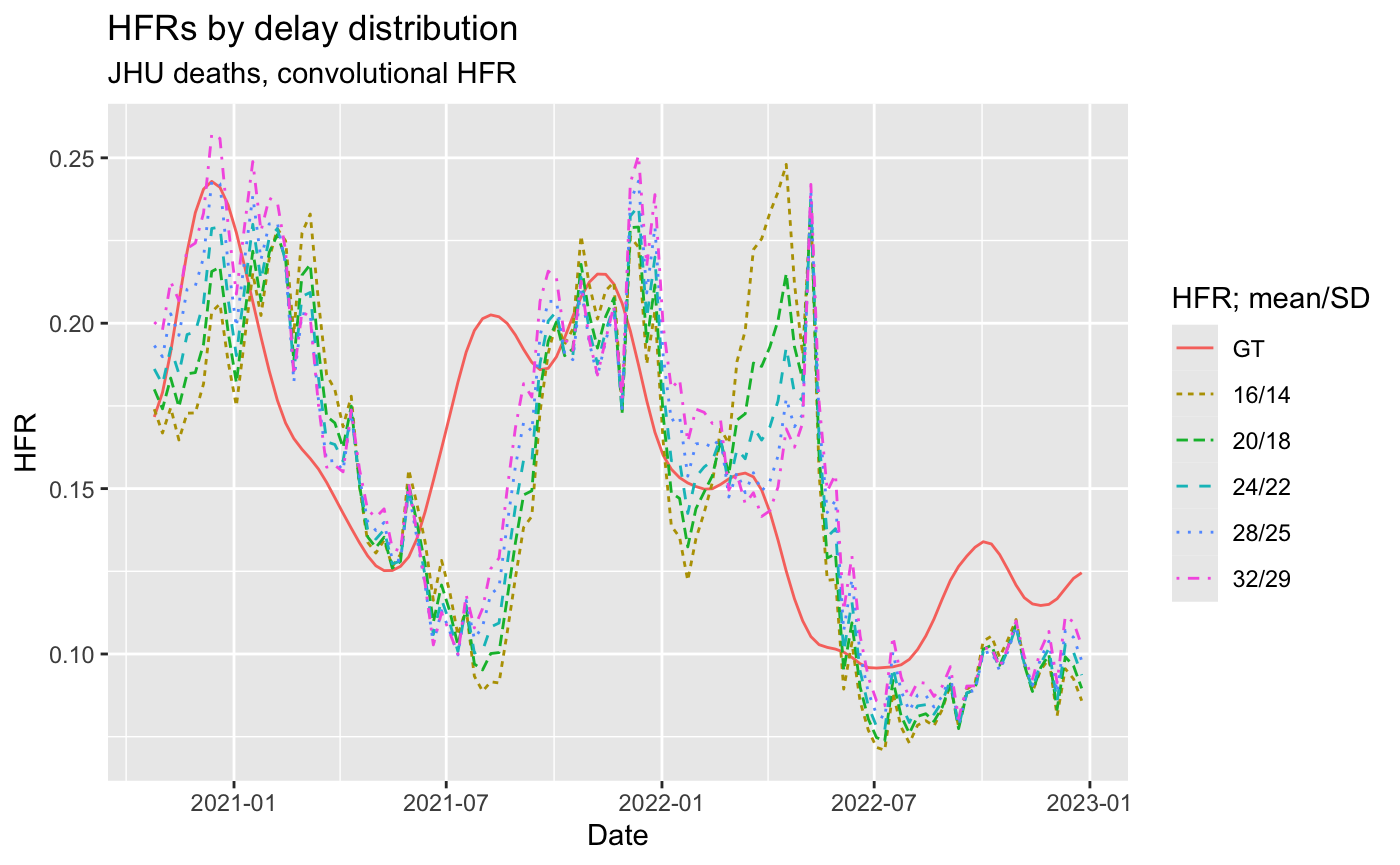
\includegraphics[width=0.7\linewidth]{Figs/Real/hfrs_by_delay.pdf}
%     \caption{HFRs are biased regardless of what delay distribution is selected.}
%     \label{fig:delay}
% \end{figure}

\begin{figure}
     \centering
     \begin{subfigure}[b]{0.45\linewidth}
         \centering
         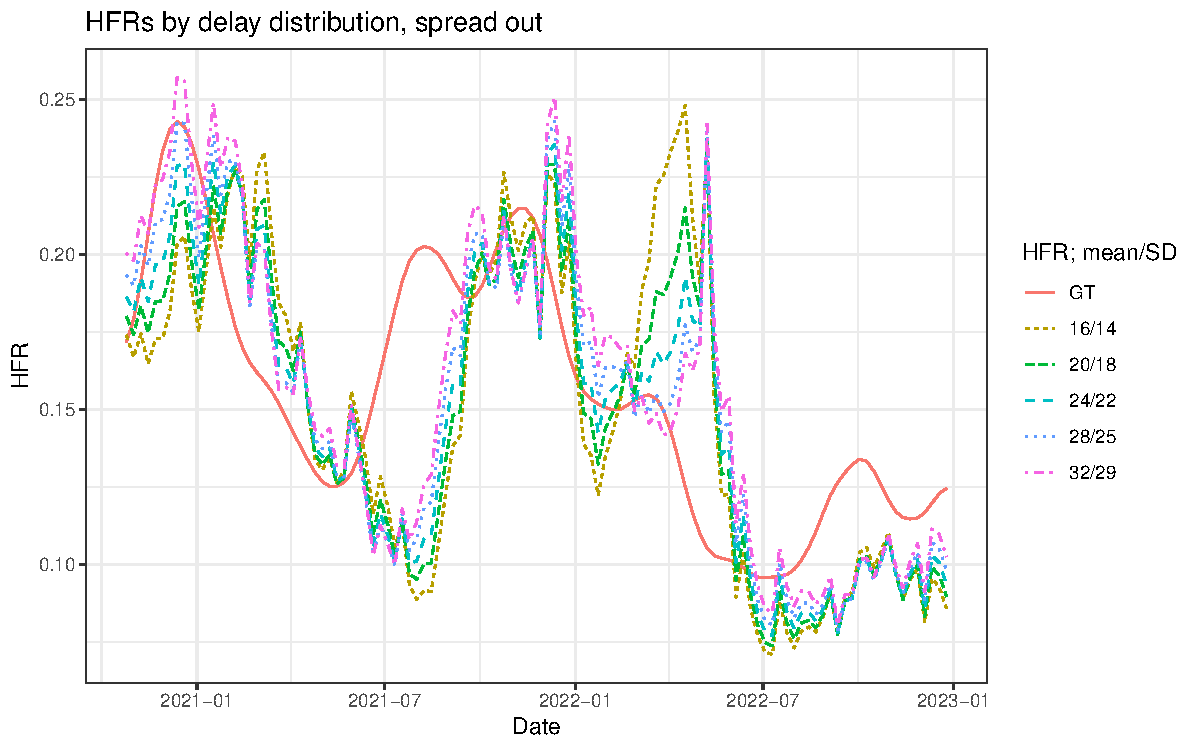
\includegraphics[width=\linewidth]{Figs/Real/hfrs_by_delay1.pdf}
         \caption{SD is $0.9\times$mean.}
         \label{fig:delay1}
     \end{subfigure}
     \hfill
     \begin{subfigure}[b]{0.45\linewidth}
         \centering
         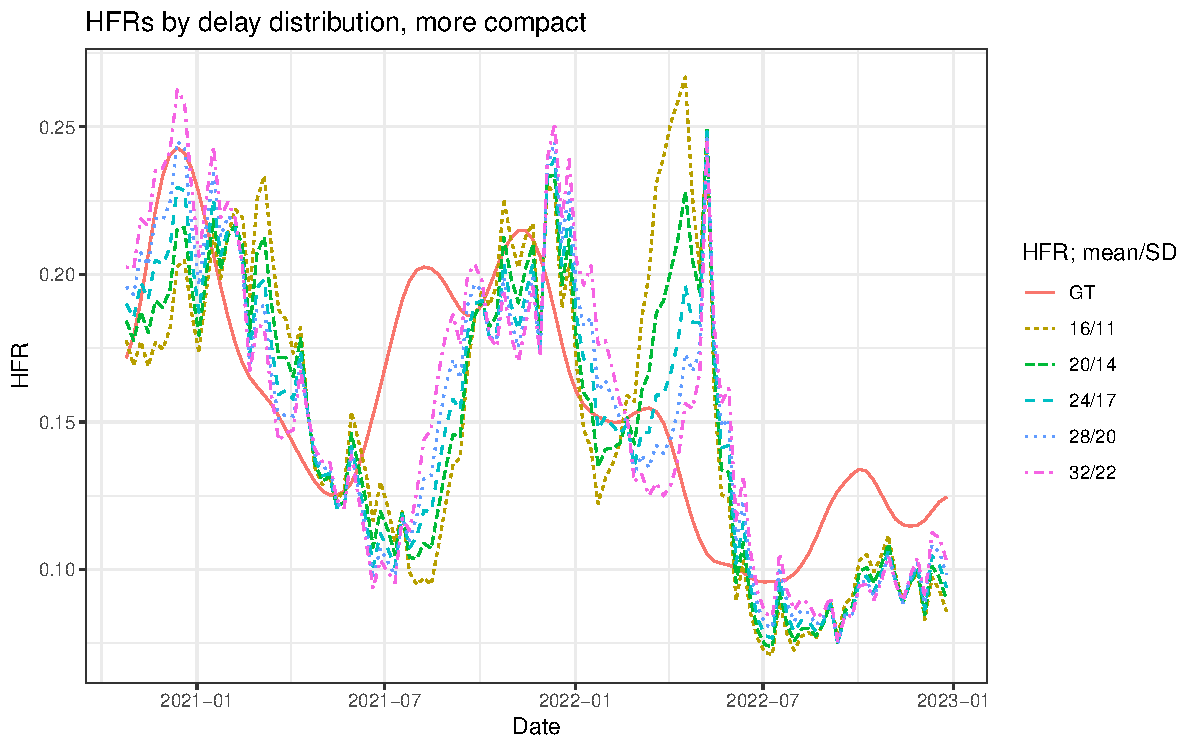
\includegraphics[width=\linewidth]{Figs/Real/hfrs_by_delay2.pdf}
         \caption{SD is $0.7\times$mean.}
         \label{fig:delay2}
     \end{subfigure}
        \caption{Convolutional ratio estimates are biased regardless of which delay distribution is selected.}
        \label{fig:delays}
\end{figure}
All HFR estimates in the figures are significantly biased. Regardless of delay distribution, the ratios are negatively biased during the onset of Delta, and surge after the peak of Omicron. This indicates the bulk of the error is fundamental to the estimator, and cannot be attributed to model misspecification. 

Comparing to the approximate ground truth HFRs from NHCS, performance improved slightly with a longer delay distribution than the purported mean of 20 days. Its mean absolute error was 0.031, whereas the delay distribution with mean 28 and standard deviation 25 had a MAE of 0.27. Nevertheless, this difference is relatively small, with the alternative delay distribution still showing similar bias.

\subsection{Geography}

Next, we repeat our analysis on different geographies, finding similar trends. We repeated our computations on the 6 largest US states with the same lag and delay distribution, with finalized death counts from JHU. Because the NHCS survey was conducted on a subset of hospitals meant to represent the US at large, it may poorly approximate the HFRs for individual states. A better state-level source is the retrospective lagged estimate (\eqref{eq:LaggedRetro}) using NCHS deaths. Figure \ref{fig:state-level} compares this rough ground truth with the real-time estimates. For both NCHS and JHU deaths, we again take the lag that maximizes cross-correlation with hospitalizations; the standard deviation of the delay distribution is 0.9 times the mean. 

 \begin{figure}
     \centering
     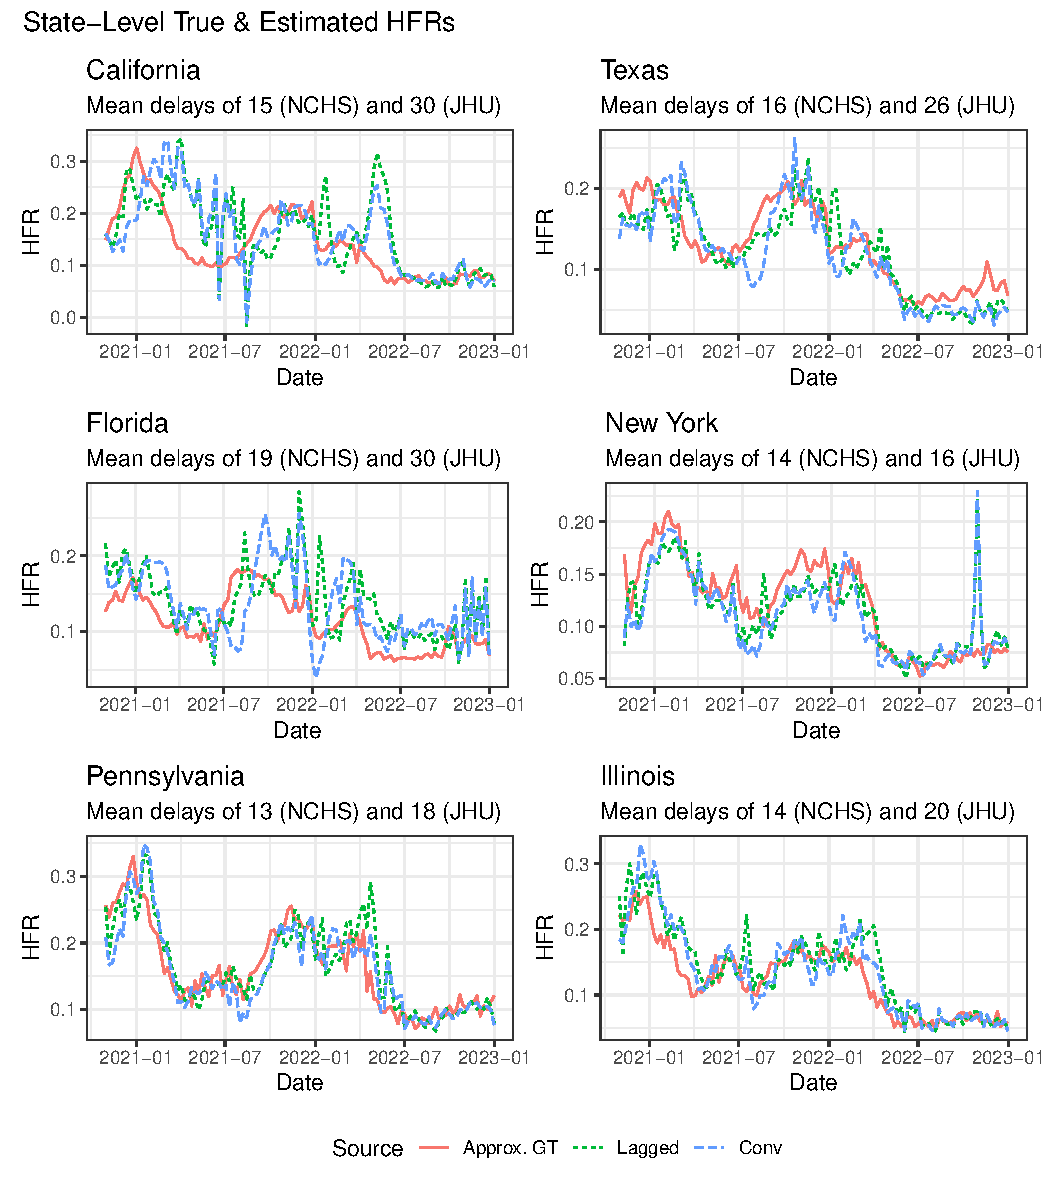
\includegraphics[width=0.8\linewidth]{Figs/Real/state_level_hfrs.pdf}
     \caption{HFRs by individual states. Comparing retrospective estimates with NCHS against real-time estimates with JHU.}
     \label{fig:state-level}
 \end{figure}

Several states have similar biases as the US results (Fig. \ref{fig:basic_est_vs_gt}). Ratios in California, Texas, and Florida all are slow to detect the uptick in HFR during Delta; in California and Florida they also spike during Omicron. Note these states are the ones with the largest optimal lags, an estimate of the average time to death. As our simulated examples have shown, the shape of the delay distribution is a key factor behind the degree of bias. In contrast, New York, Pensylvania, and Illinois have mean delays of at most 20; while their HFRs are still biased, they are relatively close to the NCHS curve. This suggests that fatality ratios are generally less trustworthy in states that take longer to report deaths.


\end{document}
